% !TeX spellcheck = de_DE
% Die erste (unkommentierte) Zeile im Dokument legt immer die
% Dokumentklasse fest
\documentclass{scrreprt} 

% Präambel:
% Einbinden von zusätzlichen Paketen. Falls für eine Datei keine Endung
% explizit angegeben wird, benutzt LaTeX '.tex'. Im Folgenden wird
% also die Datei 'edv_pakete.tex' eingebunden.
% Die erste Zeile im Dokument legt immer die Dokumentklasse fest
%\documentclass[notitlepage]{scrreprt}
    % Die wichtigsten Dokumentklassen:
    %   scrbook, scrreprt, scrartcl, beamer, standalone
    % Einige gängige Optionen für \documentclass:
    %   ngerman
    %   titlepage, notitlepage
    %   onecolumn, twocolumn
    %   oneside, twoside
    %wird in Hauptdatei festgelegt

% Präambel

% Einige KOMA-Script-Optionen
\KOMAoptions{fontsize=12pt,paper=a4}      %Schriftgröße, Papierformat
\KOMAoptions{DIV=11}                      % Parameter mit dem man den Seitenrand ändern kann
\KOMAoptions{listof=totoc}

% Hier werden einige Pakete eingebunden
\usepackage[utf8]{inputenc}               % Direkte Eingabe von ä usw. Input=Eingabe
\usepackage[T1]{fontenc}                  % Font Kodierung für die Ausgabe Font=Ausgabe
\usepackage[ngerman]{babel}               % Verschiedenste sprach-spezifische Extras, ngerman für neue deutsche Rechtschreibung, auch UK oder US möglich
\usepackage[autostyle=true]{csquotes}     % Intelligente Anführungszeichen, arbeitet mit Babel zusammen
%

\usepackage{amsmath}%Mathedarstellung
\usepackage{commath}%Mathedarstellung
\usepackage{IEEEtrantools}%IEEEeqnarray
%
\usepackage{siunitx}   % Intelligentes Setzen von Zahlen und Einheiten
\sisetup{locale = DE}  % Deutsch als locale für die Zahlen und Einheiten
%http://tex.stackexchange.com/questions/2291/how-do-i-change-the-enumerate-list-format-to-use-letters-instead-of-the-defaul

\usepackage{enumitem}%erlaubt u.A. die Aufzählung mit Buchstaben, gefunden auf http://tex.stackexchange.com/questions/2291/how-do-i-change-the-enumerate-list-format-to-use-letters-instead-of-the-defaul
%
\usepackage[varg]{txfonts}                % Schönere Schriftart, muss nach amsmath, damit keine Fehlermeldung kommt
\usepackage{graphicx} %einbinden von Figuren/Bildern
%\graphicspath{{figs/}} % Stammverzeichnis der verwendeten Bilder, muss im selben Ordner wie Hauptdatei sein
%
\usepackage[backend=biber, style=numeric, sorting=none]{biblatex}
%Verwenden von \cite in \footnote: Bibliographie drucken lassen, mehrmals kompilieren
\usepackage{hyperref}%erzeugt klickbare Elemente
\usepackage[all]{hypcap}%hyperref-befehle springen zum oberen Rand des Bildes
% Zum Einbinden von Programmcode verwenden wir das listings-Paket
\usepackage{listings}

% Für Syntax-Highlighting:
\usepackage{xcolor}
%Fuer Bilder mit gnuplot

\usepackage{color}

% Die folgenden listings-Einstellungen sind nötig, um
% deutsche Umlaute und die Tilde (~) in listings-Umgebungen
% verwenden zu können.
\lstset{
    basicstyle=\ttfamily,    
    literate={~} {$\sim$}{1} % set tilde as a literal
    {ö}{{\"o}}1
    {ä}{{\"a}}1
    {ü}{{\"u}}1
    {ß}{{\ss}}1
    {Ö}{{\"O}}1
    {Ä}{{\"A}}1
    {Ü}{{\"U}}1
}

% Farben für Code-Syntaxhighlighting und Weiteres festlegen:
\lstset{
    % Keine besondere Markierung für Leerzeichen in Codes
    showspaces=false,               
    showstringspaces=false,         
    % Farebn für Code-Kommentare und Schlüsselworte:
    commentstyle=\color{red},       % comment style
    keywordstyle=\color{blue},      % keyword style
    stringstyle=\color{orange},		% string style
    breaklines=true,
    numbers=left,                    % where to put the line-numbers; possible values are (none, left, right)
    numbersep=5pt,                   % how far the line-numbers are from the code
    stepnumber=5, 					%how often there are line numbers in code listings
    tabsize=4, 						%default tabsize set to 4 spaces
    %language=python,
    }
%gefunden auf https://en.wikibooks.org/wiki/LaTeX/Source_Code_Listings
%eigene Kommandos/Abürzungen
\newcommand{\tb}{\textbackslash}
\newcommand{\txt}{\texttt}

%Soll Zeilenumbrueche in Gleichungen vermeiden
\binoppenalty=9999
\relpenalty=9999


% Verzeichnisse mit Abbildungen; kann gestrichen werden,
% falls Sie dies schon in edv_pakete.tex definiert haben:
\graphicspath{{Bilder/}, {Bilder/Gitter/}}
\addbibresource{refsgrosschristiane.bib}

\usepackage{textcomp}
\usepackage{eurosym}

%\addbibresource{refs.bib} %Hinzufügen einer Literaturdatenbank aus dem angegebenen Verzeichnis

% Titel, Autor und Datum
\title{Monte-Carlo Simulation eines statistischen Modells auf einem Parallelrechner}
\subtitle{Bachelorarbeit in Physik}
\date{vorgelegt der Mathematisch-Naturwissenschaftlichen Fakultät der Universität Bonn \\ Juli 2020}
\author{Christiane Franziska Groß\\ angefertigt im Helmholtz-Institut für Strahlen- und Kernphysik}

% Jetzt startet das eigentliche Dokument
\begin{document}
	\maketitle
	
	% Römische Zahlen für die Seitennummern des Inhaltsverzeichnisses
	\pagenumbering{roman}
	
	Ich versichere, dass ich diese Arbeit selbstständig verfasst habe und keine anderen als die angegebenen Quellen und Hilfsmittel benutzt sowie die Zitate kenntlich gemacht habe.

	\vspace{2cm}
	
	....................................................................................
	
	\vspace{5cm}	
	
	1. Gutachter: Prof. Carsten Urbach
	
	2. Gutachter: 
	
	\newpage
	
	% Inhaltsverzeichnis kommt hier
	\tableofcontents
	
	\clearpage
	
	% Normale Zahlen für die Seitennummern des Fliesstextes
	\pagenumbering{arabic}
	%Inhalt
	
	\section*{Einleitung}
	
	
	Die vorliegende Arbeit befasst sich mit der Magnetisierung eines Magneten, der mit dem Ising-Modell in zwei Dimensionen simuliert wird. 
	
	Dazu wird erst eine kleine Einführung in die Terminologie des Ising-Modells, von Monte-Carlo-Simulationen und möglichem Aufbau von Parallelrechnern gegeben.
	
	Danach wird erläutert, wie das Modell implementiert wurde, und wie die Fehler auf die berechneten Werte bestimmt wurden.
	
	Die so erhaltenen Werte für die Magnetisierung und den kritischen Punkt werden mit den Werten, die aus der Literatur erwartet werden, verglichen. Dies wird zeigen, dass die Monte-Carlo-Simulation gut für die Simulation geeignet ist.
	
	Zusätzlich wird untersucht, wie das Programm parallelisiert werden kann, und welche Verbesserungen in der Laufzeit sich im Zuge der Parallelisierung ergeben.
	
	%Schlussendlich wird untersucht, welche Laufzeitverbesserungen durch das Rechnen mit parallelen Strukturen erzielt werden können. 
	%Ziel der Arbeit, Fragestellung: Ist MC-Simulation dafür geeignet, mittels Ising-Modell einen Magneten zu simulieren?
	
	%Wie lässt sich die benötigte Laufzeit des Programms mit Parallelisierung optimieren?/Welche Laufzeitverbesserungen sind durch Parallelisierung möglich?
	
	%Eher Zusammenfassung/abstract oder Einleitung ohne Beantwortung der Fragen?
	
	\chapter{Theoretischer Hintergrund}
	\label{chap:theorie}
	
	\section{Das Ising-Modell}
	\label{sec:isingtheorie}
	Beim Ising-Modell handelt es sich um ein Modell für einen Ferromagneten mit starker uniaxialer Anisotropie \cite[S. 7]{binderheermann}. %Hierbei werden Teilchen, die Spin $\pm 1$ haben können, auf ein quadratisches Gitter mit konstantem Abstand zwischen den Teilchen verteilt. % Gitterförmige Anordnung von Spins, die Werte $\pm1$ annehmen können, in realen Applikationen endliche Länge, in Natur thermodynamischer Limes/unendlich lang. Hier: zweidimensionales Gitter.
	
	Der Hamiltonian des Systems ist dann nach \cite[S. 7]{binderheermann}:
	\begin{equation}
	H=-J\sum_{\langle i,j\rangle }s_is_j
	\label{eq:hamiltonianising}
	\end{equation}
	Wobei $\langle i,j\rangle$ alle benachbarten Paare sind, die Austauschenergie $J$ in beide Richtungen gleich und konstant ist und die Spins $s_i$ die  Werte $\pm 1$ annehmen können. Das Vorzeichen von $J$ bestimmt, ob der Magnet ferro- oder antiferromagnetisch ist. Es ist möglich, durch einen zusätzlichen Term ein äußeres Magnetfeld zu simulieren, dies wurde in dieser Arbeit jedoch nicht getan.%Äußeres Magnetfeld möglich, aber hier vernachlässigt.

	
	%Erwarte einen kritischen Punkt mit Phasenübergang zweiter Ordnung. \cite{OnsagerCrystal1}
	Beim Ising-Modell in zwei Dimensionen wird ein Phasenübergang bei einer kritischen Temperatur erwartet, unterhalb derer sich der Magnet ferromagnetisch verhält\cite[vgl. ][]{peierls_1936}.
	
	Dieser befindet sich nach \cite{OnsagerCrystal1} bei \[\sinh^2\left(\frac{2J}{k_BT_c}\right) =1\]
	
	\begin{equation}
	\Leftrightarrow k_BT_c=\frac{2J}{\ln(1+\sqrt{2})}
	\label{eq:kritischetemperatur}
	\end{equation}
	wobei $T_c$ die kritische Temperatur und $k_B$ die Boltzmann-Konstante ist.
	
	%Magnetisierung: Erwartungswert der Spins, \[
	%M^2=\lim\limits_{m\to\infty}\left\langle s_i s_{i+m}\right\rangle \]
	
	Bei der Magnetisierung handelt es sich um den Erwartungswert der Spins, bei einem endlichen Gitter mit $N$ Punkten also\cite[vgl. ][S. 8]{binderheermann}:
	\begin{equation}
	M=\langle s \rangle=\frac{1}{N}\left\langle  \sum_{i=1}^{N} s_i \right\rangle
	\label{eq:magnetisierung}
	\end{equation}

	
	Sie ist ein Maß dafür, wie stark das Gitter nach außen als Magnet wirkt. Die erwartete Magnetisierung unterhalb des kritischen Punkt ist nach \cite{YangMagnetization}, \cite{MontrollMagnetization}:
	\begin{equation} M=\left[1-\left(\sinh\left(\frac{2J}{k_BT}\right)\right)^{-4}\right]^{\frac{1}{8}}
	\label{eq:magnetisierungsgleichungliteratur}
	\end{equation}
	
	Oberhalb der kritischen Temperatur ist die Magnetisierung null \cite[Gl. 81]{MontrollMagnetization}.
	
	Es kommt hier also zu einer Unstetigkeit in der Magnetisierung.
	
	\section{Monte-Carlo Simulationen}
	\label{sec:mctheorie}
	Die Messwerte, an denen Interesse besteht, lassen sich nach \cite[S. 8]{binderheermann}  mit \[
	\langle A(\mathbf{x}) \rangle=\frac{1}{Z}\int A(\mathbf{x}) \exp(-H(\mathbf{x})/k_BT)\dif \mathbf{x}\]
	
	\[
	Z=\int \exp(-H(\mathbf{x})/k_BT) \dif \mathbf{x}
	\]
	berechnen, wobei $\mathbf{x}$ eine mögliche Konfiguration des Systems ist.
	
	
	Hierbei kann der Boltzmann-Faktor $p(\mathbf{x})=Z^{-1} \exp(-H(\mathbf{x})/k_BT)$ als die Wahrscheinlichkeit angesehen werden, mit der ein bestimmter Zustand auftritt\cite[vgl. ][S. 8 f.]{binderheermann}.
	
	Dies ist analytisch nicht machbar, da dieses Integral sehr hochdimensional ist und gleichzeitig viele Zustände nur einen sehr kleinen Beitrag zum Gesamtintegral leisten\cite[vgl. ][S. 9]{binderheermann}.
	
	Die Idee der Monte-Carlo-Simulationen ist es, solche Integrale zu Diskretisieren
	und über alle berechneten Zustände einen Mittelwert mit Gewichtung der einzelnen Zustände mit $p(\mathbf{x})$ zu berechnen. Alternativ können die Zustände auch so gezogen werden, dass sie von Anfang an nach $p(\mathbf{x})$ verteilt sind, dann ist bei der Bildung des Mittelwerts keine Gewichtung mehr notwendig.(Zitate) %und die Zustände mit mehr Gewicht öfter zu berechnen, damit sie bei der Summierung entsprechend mehr ins Gewicht fallen. Dafür werden die zu berechnenden Zustände $A$ so gezogen, dass sie nach $Z^{-1} \exp(-H_i/k_BT)$ verteilt sind.
	
	Dies wird durch den Metropolis-Algorithmus ermöglicht, entwickelt in \cite{metropolisupdate}:
	Es wird eine Veränderung des Systems mit Energieänderung $\Delta H$ vorgeschlagen, in diesem Fall die Umdrehung eines einzelnen Spins. Diese Änderung wird auf jeden Fall angenommen, wenn sie die Energie des Systems verringert, und wenn sie die Energie erhöht, wird die Änderung mit Wahrscheinlichkeit $\exp(-\Delta H/k_BT)$ angenommen.
	
	Insgesamt ist die Wahrscheinlichkeit zur Umdrehung eines Spins also $P=\min \left[1, \exp(-\Delta H/k_BT)\right]$
	
	Dies führt dazu, dass alle zu berechnenden Zustände aus den vorher berechneten generiert werden. Die Zustände bilden also eine Markovkette, es handelt sich um Markov Chain Monte Carlo (deutsche Bezeichnung?, Zitat)
	
	Der erste Zustand wird zufällig generiert, befindet sich also nicht im Gleichgewicht und hat vermutlich ein sehr geringes Gewicht. Um in eine Region mit lokalen Energieminima/Hohen Gewichten zu kommen, ist erst eine Thermalisierung notwendig, das heißt, einige Updates, deren Ergebnisse nicht verwendet werden können, um einen Mittelwert zu bilden\cite[vgl. ][Abschnitt 3.4]{binderheermann}. %(Zitate?)
	
	Thermodynamisches Mittel=Mittel über Messungen?(Zitat)
	
%	Suche Observablen von komplexen Systemen. Problem: Zustandssumme, Observable $<A>$ nicht/nur schwer analytisch bestimmbar. \[Z=\int_{Alle Konfigurationen}\exp(-H/T)\] \[<A>=1/Z\int_{alle Konfigurationen} A\exp(-H/T)\] Generell: Integral bestimmen, nicht analytisch lösbar.
%	Idee: Diskretisiere Integral, verteile Summe nicht gleichmäßig, sondern summiere bevorzugt über Zustände, die ein höheres Gewicht haben. Zwei Funktionen Multiplizieren, Zahlen aus einer ziehen.
%%	wie Zustände generieren? Aus Zufallszahlen, nicht deterministisch, Zufallszahlen so verteilt, dass gewichtigere Zustände öfter vorkommen. Summiere über A, wobei A für Zustände mit höherem Gewicht öfter berechnet wurde.
%%	Wie Zufallszahlen generieren? Mit Markov-Kette, also aus vorherigem Zustand. Funktion zum Generieren: Metropolis-Update: Gehe von jeweils aktuellen zustand aus, schlage eine Veränderung vor(einen Spin auswählen und umdrehen), nehme an, wenn Energie kleiner wird, sonst mit Wahrscheinlichkeit $\exp(-\Delta H/T)$.
%%	
%	Am Anfang \enquote{Thermalisieren} oder Einbrennen nötig, da erst eine Region gefunden werden muss, in der die Zustände gut verteilt sind. Die Daten währen des Einbrennens werden nicht benötigt.
%	Quelle: Skript
%	\cite{binderheermann}
		
	\section{Parallelrechner}
	\label{sec:partheorie}
	Um die Berechnungen eines Standardrechner, der seriell arbeitet, zu beschleunigen, können mehrere Prozessoren oder mehrere Computer gleichzeitig an einem Programm arbeiten. Dazu gibt es zwei weit verbreitete Konzepte:
	%Parallelrechner: Durch Benutzung mehrerer Prozessorkerne oder mehrerer Computer benötigte Rechenzeit aufteilen und schneller Ergebnisse haben. Zwei Konzepte:
	\subsection{Shared Memory, hier mit OpenMP}
	\label{subsec:openmptheorie}
	Eine Möglichkeit ist, dass mehrere Prozessoren auf einen gemeinsamen Speicher zugreifen. Dies wurde in dieser Arbeit mit OpenMP umgesetzt, ein von einer nonprofit Organisation entwickelter Satz an Compilerdirektiven\cite{specificationsopenmp}.
	
	Dadurch, dass die Parallelisierung mit Compilerdirektiven umgesetzt wird, ist die Kompilierung nicht mit allen Compilern möglich. Dafür ist es aber möglich, auf einem recht hohen Abstraktionsniveau zu programmieren, ohne sich um jede Kleinigkeit beim Parallelisieren explizit zu kümmern\cite[vgl. ][S. 209]{pachecoparallel}.	
	
	In einer parallelen Region arbeiten mehrere Threads gleichzeitig an einem Teil des Programms, oder teilen sich Schleifendurchläufe auf. Hierbei kann entweder jeder Thread auf die gleichen Variablen zugreifen (shared variables) oder eine eigene Version der Variable zur Verfügung haben, die von anderen Threads nicht verändert werden kann(private variables)\cite[vgl. ][S. 231 f.]{pachecoparallel}. 
	
	Um das Verhalten der Laufzeit bei mehreren Kernen zu vergleichen, wird der Speedup gemessen:
	%Erwartetes Laufzeitverhalten bei mehr Kernen: gemessen als 
	\[\text{Speedup(n Kernen)}=\frac{\text{Laufzeit bei einem Prozessorkern}}{\text{Laufzeit bei n Prozessorkernen}}\]
	
	Naiv ist zu erwarten, dass der Sppedup linear mit der Anzahl der Kerne zunimmt. Dies berücksichtigt allerdings nicht, dass mit der Parallelisierung für jeden Kern eine zusätzliche Synchronisierung benötigt wird oder nicht alle Kerne gleichzeitig arbeiten, sondern zwischendurch auch (idle? deutsch?) sind. Daher ist zu erwarten, dass der Speedup weniger als linear zunimmt\cite[vgl. ][S. 58 f.]{pachecoparallel}.
	% linear, allerdings mehr Synchronisierungsarbeiten und anderer overhead durch parallelisierung ->. Zunahme des speedup flacht ab. (Zitat? Buch parallelisierung?) \cite{pachecoparallel}
	 
	
		
	Jede Parallelisierung führt zu mehr Overhead, also zusätzlich benötigten Rechnungen. Falls es viel Overhead gibt, wird zu dessen Ausführung genauso viel oder sogar mehr Zeit gebraucht, wie durch die Parallelisierung eingespart wurde. In diesem Fall wird der Sppedup bei höherer Anzahl an Kernen wieder kleiner.
	%Open Multi-Processing\cite{specificationsopenmp}
	%Mehrere Prozessoren greifen auf einen gemeinsamen Speicher zu, alle Prozesse können freigegebene Variablen verändern, Verhindern von Speicherproblemen durch critical-Bereiche, die nur ein Thread zu einer Zeit ausführen kann. Auch möglich, Variablen privat zu setzen, dann hat jeder Thread eine eigene Kopie der variable. Anwendung über Compiler-Pragmas\cite{tutorialopenmp}
	\subsection{MPI}
	\label{subsecmpitheorie}
	Message Passing Interface
	Mehrere Rechner mit separatem Speicher arbeiten an einem Problem, Rechner kommunizieren untereinander.
	
	
		
	\chapter{Implementierung}
	\label{chap:implementierung}
	
	\section{serielle Ausführung}
	\label{sec:seriellimplementierung}
	Bei der Implementierung des Ising-Modells auf einem Rechner müssen noch weitere Annahmen gemacht werden:
	
	Das Gitter ist nicht unendlich lang, sondern begrenzt. Je größer das Gitter ist, desto näher ist das Ergebnis am thermodynamischen Limes. 
	
	Aufgrund der Begrenzung des Gitters ist die Frage, was die Nachbarn der Teilchen am Rand des Gitters sind. Hier wurden periodische Randbedingungen gewählt, der Nachbar eines letzten Teilchen einer Zeile ist also das erste Teilchen der Spalte.
	
	Um die Auswertung der Messungen zu vereinfachen, wurde in dieser Arbeit mit $k_B=1$ gerechnet, also $T$ dimensionslos gewählt. Zudem wurde J=1 gesetzt.
	
	%Bei der Umsetzung ist nur ein endliches Gitter vorhanden.
	%Randbedingungen: Auch für die Spins am Rande des Gitters muss es Nachbarn geben. Hier wurden periodische Randbedingungen gewählt, d.h. der Nachbar von einem Punkt am Ende einer Zeile ist der Punkt am Anfang der Zeile.
	%Um Messungen zu vereinfachen: setze $k_B=1$, betrachte nur $T$.
	Bei einer Messung wird bei jedem Spin im Gitter ein Metropolis-Update durchgeführt.%Eine Messung: Bei jedem Spin wird ein Metropolis-Update durchgeführt.
	
	Dabei werden verschiedene Dinge gemessen: \begin{itemize}
		\item Der Hamiltonian des Systems, dies nach Gl.\ref{eq:hamiltonianising}
		\item Die Akzeptanzrate des Systems, also bei welchem Anteil der Spins das Metropolis-Update zur Umdrehung geführt hat. Dies wird für jedes einzelne Metropolis-Update gezählt und am Ende gemittelt.
		\item Die Magnetisierung des Systems nach Gl. \ref{eq:magnetisierung}. Aufgrund der endlichen Gitterlänge kann es vorkommen, dass das Vorzeichen der Magnetisierung während der Beobachtung wechselt. Um diesen Effekt nicht fälschlicherweise zu berücksichtigen, wird der Betrag der MAgnetisierung gemessen. \cite[vgl. ][Abschn. 2.3.3]{binderherrmann}
		%\item Das Quadrat und die vierte Potenz der Magnetisierung, um die Cumulante bestimmen zu können
	\end{itemize}
	%Akzeptanzrate: Wie viele Spins wurden bei einer Messung umgedreht? Wird bei jedem Punkt gezählt und in eine Variable geschrieben.
	
	%Magnetisierung: Betrag der Summe über alle Spins im Gitter, je mehr Spins gleich ausgerichtet sind, desto stärker der nach außen sichtbare Effekt als Magnet. Nach jeder Messung bestimmt.
	
	Das Gitter wird als eindimensionales Array abgespeichert. Das Element an Position (x,y) ist dann der laenge$\cdot$x+y-te Eintrag des Arrays (alles in C-Zählweise, also bei 0 angefangen).

	Der Hamiltonian des Gitters wird berechnet, indem das Gitter zeilenweise durchgegangen wird und von jedem Teilchen die Interaktionsenergie mit dem rechten und dem unteren Nachbarn zum bisherigen Hamiltonian addiert wird.
	
	Die zur Durchführung des Metropolis-Update benötigte Energiedifferenz bei Umdrehung eines Spin wird berechnet, indem die Energiedifferenz zu den nächsten vier Nachbarn berechnet wird. 
	Nach \cite[S. 103]{binderheermann} kann diese Energiedifferenz nur einer von fünf Werten sein. Daher wird die Wahrscheinlichkeit für die Spindrehung nicht jedes mal neu berechnet, sondern in einem Array nachgeschaut.
	
	Um zu erreichen, dass der Spinflip mit der entsprechenden Wahrscheinlichkeit angenommen wird, wird die Wahrscheinlichkeit mit einer Zufallszahl zwischen null und eins verglichen\cite[nach][]{metropolisupdate}. Wenn die Wahrscheinlichkeit größer als die Zufallszahl ist, wird der Spinflip ausgeführt, und die Energiedifferenz zum Hamiltonian dazu addiert
	
	Die Messung wird in der sweep-Funktion durchgeführt, in der in for-Schleifen das ganze Gitter durchgegangen wird. Für jeden Punkt wird die Energiedifferenz bei Umdrehung ermittelt und damit ein Metropolis-Update durchgeführt. Nachdem bei jedem Punkt ein Update durchgeführt worden ist, wird die Akzeptanzrate sowie die Magnetisierung in eine .txt-Datei ausgegeben, in der die Ergebnisse aller Messungen gespeichert werden.
	%Hamiltonian: berechnen über zeilenweise Array durchgehen, von jedem Punkt rechten und unteren Nachbarn, periodische Randbedingungen durch modulo.
	%Metropolis-Update: Nur vier Nachbarn zum Berechnen nötig, Hamiltonian wird als Parameter übergeben, daraus Änderung bei Flip, Akzeptanz wird durch 0/1 zurückgegeben. Wahrscheinlichkeit für Flip: Vergleich mit Zufallszahl zwischen null und eins.
	%sweep Funktion: geht das ganze Gitter durch und führt bei jedem Punkt ein Metropolis-Update durch. Zählt wie viele Spins geflippt werden, schreibt am Ende Prozentuale Veränderungen (Akzeptanzrate) und Summe über alle Spins(Magnetisierung) in Ausgabedatei.
	
	Um eine zufällige Anfangskonfiguration zu erzeugen, wird ein eindimensionales Array mit laenge$\cdot$laenge Einträgen erstellt. Mithilfe von Zufallszahlen aus der Gnu Scientific Library \cite{gsldoc} wird jedem Element des Arrays zufällig $1$ oder $-1$ zugeteilt.	
	%Initialisierung des Gitters: Als 1D Array abspeichern, mit Mersenne Twister $\pm1$ auf das Gitter verteilen.
	
	Diese zufällige Konfiguration ist weit vom interessanten Gleichgewicht entfernt, sodass die ersten Messungen nicht verwendet werden können. Daher ist am Anfang eine Thermalisierung nötig, nach der sich das System im Gleichgewicht befindet. Für die erste Temperatur werden (10.000) Messungen durchgeführt und verworfen, für alle Temperaturen danach wird das Gitter der vorherigen Temperatur übergeben und mit (5.000) Messungen thermalisiert. Das thermalisierte Gitter wird ausgegeben und kann somit auch für spätere Messungen wieder verwendet werden. Die Datei mit den Messergebnissen der Thermalisierung ist nicht relevant.
	
	Beim Messen wird die gewünschte Anzahl an Messungen als Parameter übergeben, die Messungen werden in eine Datei geschrieben.
	
	%Am Anfang Einbrennen nötig: Gitter der vorherigen Temperatur wird übergeben, N0 (=10.000) Messungen werden durchgeführt, deren Ergebnisse nicht verwendet werden, da sie zu stark variieren, Gitter nach Einbrennen wird in .txt Datei gespeichert.
	
	%Danach messen: Ergebnisse werden in Ausgabedatei geschrieben.
	
	Die Daten der Messdatei werden wieder eingelesen, um daraus den naiven Mittelwert $\mu=\frac{1}{N}\sum_{i} x_i$ und die naive Standardabweichung $\sigma=\frac{1}{N-1}\sum_{i}(x_i-\mu)^2$ zu bilden. Diese werden zusammen mit Temperatur und Gitterlänge in eine Datei geschrieben.
	%Aus Datei durch einlesen mit Standardschätzern naiven Mittelwert $\mu=\frac{1}{N}\sum_{i} x_i$ bilden und damit Standardabweichung $\sigma=\frac{1}{N-1}\sum_{i}(x_i-\mu)^2$ berechnen. Temperatur, Mittelwert und Varianz der Akzeptanzrate und Magnetisierung werden in Datei geschrieben.
	
	Da es sich um Markov-Chain-Monte-Carlo handelt, sind die Konfigurationen nicht voneinander unabhängig, also autokorreliert. Insbesondere ist diese Autokorrelation temperaturabhängig(warum? Zitat).
	
	Um die Autokorrelation zu verringern, werden die Mittelwerte und Fehler der Messdaten zusätzlich noch durch Bootstrapping mit vorherigem Blocking bestimmt. Das Blocking sorgt dafür, dass die Autokorrelation kleiner wird, dass Bootstrapping dafür, dass die ermittelten Werte eher der zugrundeliegenden Wahrscheinlichkeitsverteilung entsprechen. Die Werte zur Erzeugung der Blöcke werden wiederum aus der .txt-Datei mit den Messergebnissen eingelesen.
	
%	Fehler kommen durch Autokorrelation der Daten, sind also Temperaturabhängig: Beseitigung der Autokorrelation durch Blocking der Daten, also Einteilen in verschiedene Blöcke der Länge $l$, danach Bootstrapping, um Fehlerqualität zu verbessern. (Zitat?)
	%Bootstrapping: zur Erzeugung eines Replikas aus Messwerten so viele Werte mit Zurücklegen ziehen, wie es Messungen gibt und daraus den arithmetischen Mittelwert bilden. Aus $r$ so gebildeten Replikas den Standardschätzer für Mittelwert und Varianz ziehen. Temperatur, $l$, Mittelwert und Varianz in Datei schreiben.
	
	Der so berechnete Fehler hängt von der Länge l der Blöcke ab, er steigt mit der Länge. Ab einer gewissen Länge bleiben die Fehler konstant, diese Region eignet sich gut, um temperaturunabhängige Fehler zu bestimmen.
	%So errechneter Fehler steigt mit l an, ab einer gewissen Länge bildet sich ein Plateau. Quelle: Skript.
	
	Bild Fehler in Abhängigkeit von l? ERklärung Bootstrapping? Zitate?
	
	Zur Bestimmung des kritischen Punktes wird ausgenutzt, dass an diesem eine Unstetigkeit in der Ableitung bestehen sollte. Aufgrund der endlichen Länge des Gitters, gibt es keine Unstetigkeit, sondern nur ein Extremum. Dieses wird bestimmt, indem das Maximum der mit der 2-Punkt-Formel gebildeten Ableitung bestimmt wird. Der Fehler der Ableitung wird mittels Gaußscher Fehlerfortpflanzung bestimmt.
	%Kritischer Punkt: Unstetigkeit in Magnetisierung/Pol in Ableitung erwartet, bestimmen über größte Änderung/Extremum der Ableitung der Magnetisierung: Mit 2-Punkt-Formel berechnete Ableitung, Fehler der Ableitung mit Gaußscher Fehlerfortpflanzung ermittelt.
		
	Um die Magnetisierung bei vielen Temperaturen zu messen, werden in der main-funktion Variablen wie J und ein Array für die Temperaturen initialisiert. Außerdem wird die Anzahl an Messungen, Thermalisierungsschritten vor der ersten Temperatur, Thermalisierungsschritten vor jeder Temperatur sowie die Blocklänge fürs Bootstrapping festgelegt. 	
	%Main-funktion: Variablen wie T, J, N0 initialisieren, Array mit verwendeten Temperaturen und l fürs Bootstrapping erzeugen, Dateien für Mittelwerte öffnen
	
	Zuerst wird ein Gitter erstellt, initialisiert und zum ersten Mal bei der niedrigsten betrachteten Temperatur thermalisiert. Danach werden in einer for-Schleife alle gewählten Temperaturen aufsteigend bearbeitet, bei jeder Temperatur wird das Gitter erst thermalisiert und danach die gewünschte Zahl an Messungen durchgeführt.
	%Messungen für verschiedene Temperaturen: Durch for-Schleife, vorher Initialisierung eines Array, in das die Temperaturen gleichmäßig verteilt hineingeschrieben werden.
	Die Messergebnisse werden in einer .txt-Datei gespeichert. Danach wird aus den Messwerten sowohl mit der naiven Methode, als auch mit Blocking und Bootstrapping, der Mittelwert sowie die Standardabweichung der Magnetisierung(, der Akzeptanzrate und des Hamiltonians) bei der gegebenen Temperatur bestimmt.
	%Initialisierung mit (100.000) Messungen am ersten Gitter, danach Thermalisierung mit Gitter der vorherigen Temperatur.
	%for-Schleife über alle Temperaturen im array: Datei für Gitter, Messergebnisse öffnen, thermalisieren, messen, naive Schätzer und Bootstrapschätzer für verschiedene l bestimmen.
	
	Am Ende des Programms wird aus den ermittelten Werten die Ableitung der Magnetisierung berechnet und ebenfalls in eine .txt-Datei geschrieben.
	%Am Ende Ableitung in separate Datei schreiben.
		
	
	\section{parallele Ausführung}
	\label{sec:parallelimplementierung}


	
	Die zum Messen benötigte Zeit steigt mit dem Quadrat der Gitterlänge. Dies sorgt vor allem bei den interessanten langen Gitterlängen, die näher an den thermodynamischen Limes herankommen, für lange Messzeiten. Um diese Messungen zu beschleunigen, wurde das Programm parallelisiert.
	
	Im ersten Schritt der Parallelisierung, mit OpenMP, wurden rechenintensive for-Schleifen parallelisiert.
	%Einzelne Messung dauert recht lange: Beschleunigen durch parallelisieren. 
	%Strategie: Vor allem Rechenintensive Bereiche parallelisieren, z.B. sweep-funktion für Messvorgang und Replikas ziehen.
	%Parallelisiert: for-Schleifen, deren Ausführungen unabhängig vom vorherigen Schleifendurchgang sind.
	
	
	\begin{wrapfigure}{r}{3.5in}
		%\begin{figure}[htbp]
		\centering
		% GNUPLOT: LaTeX picture with Postscript
\begingroup
  \makeatletter
  \providecommand\color[2][]{%
    \GenericError{(gnuplot) \space\space\space\@spaces}{%
      Package color not loaded in conjunction with
      terminal option `colourtext'%
    }{See the gnuplot documentation for explanation.%
    }{Either use 'blacktext' in gnuplot or load the package
      color.sty in LaTeX.}%
    \renewcommand\color[2][]{}%
  }%
  \providecommand\includegraphics[2][]{%
    \GenericError{(gnuplot) \space\space\space\@spaces}{%
      Package graphicx or graphics not loaded%
    }{See the gnuplot documentation for explanation.%
    }{The gnuplot epslatex terminal needs graphicx.sty or graphics.sty.}%
    \renewcommand\includegraphics[2][]{}%
  }%
  \providecommand\rotatebox[2]{#2}%
  \@ifundefined{ifGPcolor}{%
    \newif\ifGPcolor
    \GPcolortrue
  }{}%
  \@ifundefined{ifGPblacktext}{%
    \newif\ifGPblacktext
    \GPblacktextfalse
  }{}%
  % define a \g@addto@macro without @ in the name:
  \let\gplgaddtomacro\g@addto@macro
  % define empty templates for all commands taking text:
  \gdef\gplbacktext{}%
  \gdef\gplfronttext{}%
  \makeatother
  \ifGPblacktext
    % no textcolor at all
    \def\colorrgb#1{}%
    \def\colorgray#1{}%
  \else
    % gray or color?
    \ifGPcolor
      \def\colorrgb#1{\color[rgb]{#1}}%
      \def\colorgray#1{\color[gray]{#1}}%
      \expandafter\def\csname LTw\endcsname{\color{white}}%
      \expandafter\def\csname LTb\endcsname{\color{black}}%
      \expandafter\def\csname LTa\endcsname{\color{black}}%
      \expandafter\def\csname LT0\endcsname{\color[rgb]{1,0,0}}%
      \expandafter\def\csname LT1\endcsname{\color[rgb]{0,1,0}}%
      \expandafter\def\csname LT2\endcsname{\color[rgb]{0,0,1}}%
      \expandafter\def\csname LT3\endcsname{\color[rgb]{1,0,1}}%
      \expandafter\def\csname LT4\endcsname{\color[rgb]{0,1,1}}%
      \expandafter\def\csname LT5\endcsname{\color[rgb]{1,1,0}}%
      \expandafter\def\csname LT6\endcsname{\color[rgb]{0,0,0}}%
      \expandafter\def\csname LT7\endcsname{\color[rgb]{1,0.3,0}}%
      \expandafter\def\csname LT8\endcsname{\color[rgb]{0.5,0.5,0.5}}%
    \else
      % gray
      \def\colorrgb#1{\color{black}}%
      \def\colorgray#1{\color[gray]{#1}}%
      \expandafter\def\csname LTw\endcsname{\color{white}}%
      \expandafter\def\csname LTb\endcsname{\color{black}}%
      \expandafter\def\csname LTa\endcsname{\color{black}}%
      \expandafter\def\csname LT0\endcsname{\color{black}}%
      \expandafter\def\csname LT1\endcsname{\color{black}}%
      \expandafter\def\csname LT2\endcsname{\color{black}}%
      \expandafter\def\csname LT3\endcsname{\color{black}}%
      \expandafter\def\csname LT4\endcsname{\color{black}}%
      \expandafter\def\csname LT5\endcsname{\color{black}}%
      \expandafter\def\csname LT6\endcsname{\color{black}}%
      \expandafter\def\csname LT7\endcsname{\color{black}}%
      \expandafter\def\csname LT8\endcsname{\color{black}}%
    \fi
  \fi
    \setlength{\unitlength}{0.0500bp}%
    \ifx\gptboxheight\undefined%
      \newlength{\gptboxheight}%
      \newlength{\gptboxwidth}%
      \newsavebox{\gptboxtext}%
    \fi%
    \setlength{\fboxrule}{0.5pt}%
    \setlength{\fboxsep}{1pt}%
\begin{picture}(5040.00,5040.00)%
    \gplgaddtomacro\gplbacktext{%
      \csname LTb\endcsname%
      \put(2356,4401){\makebox(0,0){\strut{}}}%
    }%
    \gplgaddtomacro\gplfronttext{%
      \csname LTb\endcsname%
      \put(630,103){\makebox(0,0){\strut{}$0$}}%
      \put(1397,103){\makebox(0,0){\strut{}$2$}}%
      \put(2165,103){\makebox(0,0){\strut{}$4$}}%
      \put(2931,103){\makebox(0,0){\strut{}$6$}}%
      \put(3699,103){\makebox(0,0){\strut{}$8$}}%
      \put(250,3888){\makebox(0,0)[r]{\strut{}$0$}}%
      \put(250,3157){\makebox(0,0)[r]{\strut{}$2$}}%
      \put(250,2426){\makebox(0,0)[r]{\strut{}$4$}}%
      \put(250,1696){\makebox(0,0)[r]{\strut{}$6$}}%
      \put(250,965){\makebox(0,0)[r]{\strut{}$8$}}%
    }%
    \gplbacktext
    \put(0,0){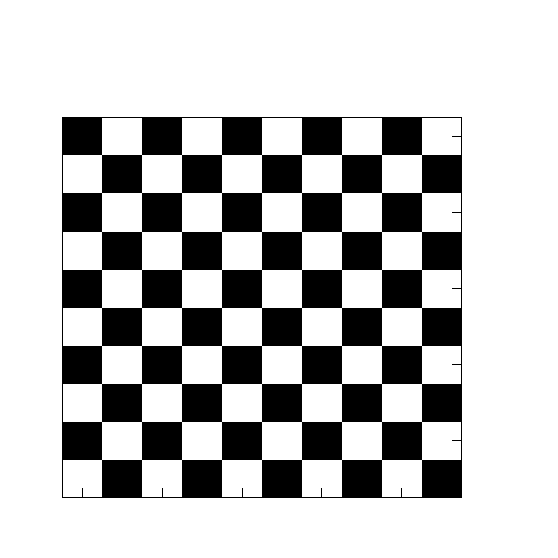
\includegraphics{schachbrett}}%
    \gplfronttext
  \end{picture}%
\endgroup

		\label{fig:schachbrett}
		\caption{Schachbrettmuster}
		%\end{figure}
	\end{wrapfigure}
	
	Insbesondere bei der sweep-Funktion, die bei jedem Spin ein Metropolis-Update durchführt, lohnt sich eine Parallelisierung. Hierfür müssen jedoch die einzelnen Schleifendurchführungen unabhängig voneinander sein. Dies ist beim einfachen zeilenweise Durchgehen nicht der Fall.
	Um die einzelnen Schleifendurchläufe unabhängig voneinander zu machen, wird das Gitter in zwei Untergitter aufgeteilt, die nacheinander abgearbeitet werden. Dies ist möglich, da für ein Update nur benötigt wird, das die vier direkten Nachbarn unverändert sind. Daher lässt sich das Gitter in \enquote{schwarze}
	und \enquote{weiße} Punkte aufteilen, ähnlich einem Schachbrettmuster in Abb. \ref{fig:schachbrett}. Um ein Update an einem \enquote{schwarzen} Punkt durchzuführen, werden nur \enquote{weiße} Punkte benötigt und umgekehrt. Die schwarzen Punkte sind dadurch definiert, dass die Summe der Koordinaten eine gerade Zahl ist, die Summe der Koordinaten der weißen Punkte ist ungerade.
	
	Die Parallelisierung von for-Schleifen ist in OpenMP eingebaut und wird durch Compiler-Pragmas eingebaut. In jedem Schleifendurchlauf wird die Akzeptanzrate sowie die Änderung des Hamiltonians gemessen. Bei der Parallelisierung ist es wichtig, dass nicht mehrere Threads gleichzeitig versuchen, eine Variable zu verändern. Deshalb werden die entsprechenden Variablen als privat deklariert, sodass jeder Thread eine eigene Kopie der Variable bekommt. Erst am Ende der Messung werden ein einer kritischen Region, die nur ein Thread zu einer Zeit durchführen kann, werden die Änderungen zusammengeführt. 	%sweep: bei zeilenweise durchgehen des Gitters von vorheriger Änderung abhängig.
	%Unabhängig: Gitter wie Schachbrett sehen, Update der Schwarzen Felder hängt nur von weißen ab und umgekehrt. Aufspalten in zwei separate for-Schleifen, eine Farbe pos1+pos2 gerade, andere ungerade. Einzelne Schleifen parallelisieren, Updates von Hamiltonian/Anzahl der geänderten Variablen in eigene Zwischenvariablen, Updaten in einer critical region(nur ein Thread kann Region zu einer Zeit ausführen) am Ende der Schleife.
	
	%Replikas ziehen: Gezogene Replikas werden in array geschrieben: Vollkommen unabhängig, parallelisieren der for-Schleife.
	
	Zusätzlich ist es wichtig, dass jeder Thread auf einen eigenen Zufallszahlengenerator zugreift. Dies lässt sich nicht durch die Deklarierung des Generators als privat erreichen, sondern wird dadurch erreicht, dass nicht ein einzelner Generator, sondern ein Array von Generatoren als Parameter an die sweep-Funktion übergeben wird.
	
	In der seriellen Ausführung der sweep-Funktion sind zwei ineinander geschachtelte for-Schleifen, die dafür sorgen, dass das gesamte Gitter einmal zeilenweise durchgegangen wird.
	
	In der parallelen Funktion wurde dies durch zwei Schleifenpaare ersetzt, eins für die schwarzen Punkte und eins für die weißen Punkte.
	
	Dafür wurden die Schleifenköpfe des seriellen Durchgangs so modifiziert, dass in jeder Zeile nur bei jedem zweiten Punkt ein Metropolis-Update durchgeführt wird. 
	\begin{verbatim}
	for (d1=0; d1<laenge;d1+=1){
		for (d2=(d1%2); d2<laenge; d2+=2){
	\end{verbatim}
	Hierbei sind \texttt{d1} und \texttt{d2} die Koordinaten und \texttt{laenge} die Länge des Gitters. Dadurch, dass die zweite Schlefe mithilfe eines Modulo-Operators initialisiert wird, springt für jede Zeile die Position der betrachteten Punkte, wie es für ein Schachbrettmuster nötig ist. Um die weißen Punkte zu betrachten, wurde \texttt{(d1\%2)} durch \texttt{((d1+1)\%2)} ersetzt.
	% Auch in diesen Schleifen wird das ganze Gitter abgegangen, um Schleifendurchläufe zu verhindern, bei denen die Punkte der falschen Farbe untersucht werden, wird in der inneren Schleife nur jeder zweite Punkt berücksichtigt.
	%Statt einer Schleife zwei, andere Initialisierung für schwarz/weiß
	
	Jede Parallelisierung führt zu mehr Overhead, also zusätzlich benötigten Rechnungen. Falls es viel Overhead gibt, wird zu dessen Ausführung genauso viel oder sogar mehr Zeit gebraucht, wie durch die Parallelisierung eingespart wurde.
	
	Deshalb wurden einige Funktionen, die zwar gut parallelisierbar wären, wie z.B die Berechnung des Hamiltonians oder die Berechnung der Summe über alle Gitterelemente, nicht parallelisiert.
	

	%Zeitersparnis Tabelle/Grafik Nummer an Kernen/Gebrauchte Zeit. Auch für einzelne Funktionen?
	%Funktion parallelisiert, die Summe über das Gitter berechnet: Zeitersparnis nur 0,5\%, daher Hamiltonian, einmaliges Verteilen der Zufallszahlen auf Gitter nicht parallelisiert.
	

	
	 	
	\chapter{Ergebnisse}
	\label{chap:ergebnisse}
	
	Zuerst wird sichergestellt, dass das Programm sowohl bei paralleler als auch bei serieller Ausführung das gleiche Verhalten aufweist. Wie man an Bild \ref{fig:vergleichham} sieht, ist das der Fall, die Ergebnisse liegen aufeinander und sind insbesondere in ihren Fehlergrenzen gleich.
	
	\begin{figure}[htbp]
		% GNUPLOT: LaTeX picture with Postscript
\begingroup
  \makeatletter
  \providecommand\color[2][]{%
    \GenericError{(gnuplot) \space\space\space\@spaces}{%
      Package color not loaded in conjunction with
      terminal option `colourtext'%
    }{See the gnuplot documentation for explanation.%
    }{Either use 'blacktext' in gnuplot or load the package
      color.sty in LaTeX.}%
    \renewcommand\color[2][]{}%
  }%
  \providecommand\includegraphics[2][]{%
    \GenericError{(gnuplot) \space\space\space\@spaces}{%
      Package graphicx or graphics not loaded%
    }{See the gnuplot documentation for explanation.%
    }{The gnuplot epslatex terminal needs graphicx.sty or graphics.sty.}%
    \renewcommand\includegraphics[2][]{}%
  }%
  \providecommand\rotatebox[2]{#2}%
  \@ifundefined{ifGPcolor}{%
    \newif\ifGPcolor
    \GPcolortrue
  }{}%
  \@ifundefined{ifGPblacktext}{%
    \newif\ifGPblacktext
    \GPblacktextfalse
  }{}%
  % define a \g@addto@macro without @ in the name:
  \let\gplgaddtomacro\g@addto@macro
  % define empty templates for all commands taking text:
  \gdef\gplbacktext{}%
  \gdef\gplfronttext{}%
  \makeatother
  \ifGPblacktext
    % no textcolor at all
    \def\colorrgb#1{}%
    \def\colorgray#1{}%
  \else
    % gray or color?
    \ifGPcolor
      \def\colorrgb#1{\color[rgb]{#1}}%
      \def\colorgray#1{\color[gray]{#1}}%
      \expandafter\def\csname LTw\endcsname{\color{white}}%
      \expandafter\def\csname LTb\endcsname{\color{black}}%
      \expandafter\def\csname LTa\endcsname{\color{black}}%
      \expandafter\def\csname LT0\endcsname{\color[rgb]{1,0,0}}%
      \expandafter\def\csname LT1\endcsname{\color[rgb]{0,1,0}}%
      \expandafter\def\csname LT2\endcsname{\color[rgb]{0,0,1}}%
      \expandafter\def\csname LT3\endcsname{\color[rgb]{1,0,1}}%
      \expandafter\def\csname LT4\endcsname{\color[rgb]{0,1,1}}%
      \expandafter\def\csname LT5\endcsname{\color[rgb]{1,1,0}}%
      \expandafter\def\csname LT6\endcsname{\color[rgb]{0,0,0}}%
      \expandafter\def\csname LT7\endcsname{\color[rgb]{1,0.3,0}}%
      \expandafter\def\csname LT8\endcsname{\color[rgb]{0.5,0.5,0.5}}%
    \else
      % gray
      \def\colorrgb#1{\color{black}}%
      \def\colorgray#1{\color[gray]{#1}}%
      \expandafter\def\csname LTw\endcsname{\color{white}}%
      \expandafter\def\csname LTb\endcsname{\color{black}}%
      \expandafter\def\csname LTa\endcsname{\color{black}}%
      \expandafter\def\csname LT0\endcsname{\color{black}}%
      \expandafter\def\csname LT1\endcsname{\color{black}}%
      \expandafter\def\csname LT2\endcsname{\color{black}}%
      \expandafter\def\csname LT3\endcsname{\color{black}}%
      \expandafter\def\csname LT4\endcsname{\color{black}}%
      \expandafter\def\csname LT5\endcsname{\color{black}}%
      \expandafter\def\csname LT6\endcsname{\color{black}}%
      \expandafter\def\csname LT7\endcsname{\color{black}}%
      \expandafter\def\csname LT8\endcsname{\color{black}}%
    \fi
  \fi
    \setlength{\unitlength}{0.0500bp}%
    \ifx\gptboxheight\undefined%
      \newlength{\gptboxheight}%
      \newlength{\gptboxwidth}%
      \newsavebox{\gptboxtext}%
    \fi%
    \setlength{\fboxrule}{0.5pt}%
    \setlength{\fboxsep}{1pt}%
\begin{picture}(8640.00,6480.00)%
    \gplgaddtomacro\gplbacktext{%
      \csname LTb\endcsname%
      \put(946,704){\makebox(0,0)[r]{\strut{}$-2.2$}}%
      \put(946,1316){\makebox(0,0)[r]{\strut{}$-2$}}%
      \put(946,1929){\makebox(0,0)[r]{\strut{}$-1.8$}}%
      \put(946,2541){\makebox(0,0)[r]{\strut{}$-1.6$}}%
      \put(946,3153){\makebox(0,0)[r]{\strut{}$-1.4$}}%
      \put(946,3766){\makebox(0,0)[r]{\strut{}$-1.2$}}%
      \put(946,4378){\makebox(0,0)[r]{\strut{}$-1$}}%
      \put(946,4990){\makebox(0,0)[r]{\strut{}$-0.8$}}%
      \put(946,5603){\makebox(0,0)[r]{\strut{}$-0.6$}}%
      \put(946,6215){\makebox(0,0)[r]{\strut{}$-0.4$}}%
      \put(1078,484){\makebox(0,0){\strut{}$0$}}%
      \put(2511,484){\makebox(0,0){\strut{}$1$}}%
      \put(3944,484){\makebox(0,0){\strut{}$2$}}%
      \put(5377,484){\makebox(0,0){\strut{}$3$}}%
      \put(6810,484){\makebox(0,0){\strut{}$4$}}%
      \put(8243,484){\makebox(0,0){\strut{}$5$}}%
    }%
    \gplgaddtomacro\gplfronttext{%
      \csname LTb\endcsname%
      \put(176,3459){\rotatebox{-270}{\makebox(0,0){\strut{}$H/\text{laenge}^2$}}}%
      \put(4660,154){\makebox(0,0){\strut{}Temperatur}}%
      \csname LTb\endcsname%
      \put(4642,6042){\makebox(0,0)[r]{\strut{}zeilenweise durchgehen}}%
      \csname LTb\endcsname%
      \put(4642,5822){\makebox(0,0)[r]{\strut{}Schachbrettmuster parallel}}%
    }%
    \gplbacktext
    \put(0,0){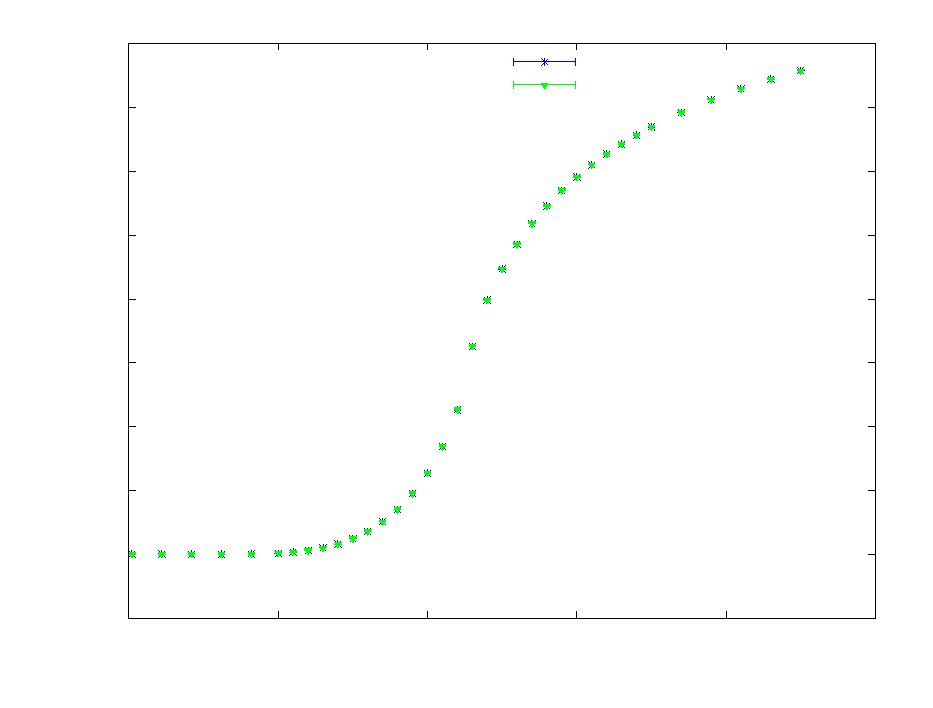
\includegraphics{vergleichham}}%
    \gplfronttext
  \end{picture}%
\endgroup

		\label{fig:vergleichham}
		\caption[Hamiltonian mit und ohne Parallelisierung]{Hamiltonian mit und ohne Parallelisierung bei verschiedenen Temperaturen gemessen. Die Fehler sind mit Blocklänge 128 bestimmt und so klein, dass sie fast nicht sichtbar sind.}
	\end{figure}
	
	Um zu ermitteln, mit wie vielen Cores idealerweise gemessen werden sollte, wurde die Skalierung der sweep-Funktion betrachtet. Hierbei wurde für verschiedene Gitterlängen und Temperaturen die Zeit, die für 10.000 Ausführungen der sweep-Funktion benötigt wurde, gemessen. 
	
	Wie man an Bild sieht, ist die Parallelisierung für kleine Gitterlängen sinnlos, es wird nur mehr overhead eingeführt und die benötigte Zeit steigt mit Anzahl der Cores.
	
	Ab einer gewissen Gitterlänge sinkt die benötigte Rechenzeit mit mehr Cores, sinkt allerdings für mehr Cores, wenn es mehr Overhead gibt. Bei steigender Gitterlänge wird allerdings auch die Laufzeitverbesserung für mehr Cores sichtbar, es bildet sich erst ein Plateau, was für lange Gitterlängen schließlich in eine monoton steigende Funktion übergeht.
	
	Wenn man sich die Skalierung bei verschiedenen Temperaturen anguckt, gibt es auch hier Unterschiede bei konstanter Gitterlänge: für niedrigere Temperaturen ist die Laufzeit geringer, allerdings der maximale speedup kleiner. Vermutlich kommt dies daher, dass bei niedrigen Temperaturen die Akzeptanzrate geringer ist und somit seltener eine Addition beim Hamiltonian durchgeführt werden muss.
	
	Bei Gitterlängen ab  entspricht das Ergebnis somit den Erwartungen aus Abschnitt \ref{subsec:openmptheorie}
	%Insgesamt entspricht somit die Skalierung bei hohen Gitterlängen dem Ahmdahlschen Gesetz.
	Messungen der Parallelisierung von messen/sweep auf lcpunode02 in QBiG: Bis zu 12 Kerne. Kennwerte von lcpunode02?
	%Parallelisierung Bootstrap?
	
	%Zuerst: Vergleich der verschiedenen sweep-Funktionen: Hamiltonian gleich. Bild.
	
	%Skalierung auf lcpunode2: Vergleich zwei Schleifen/tryflip/Temperaturen?
	%Bild von idealem Code, Skalierung wie erwartet (nach Ahmdahls law?)
	
	In Bild \ref{fig:ergebnisakzeptanzrate} ist die Akzeptanzrate als Funktion von der Temperatur dargestellt. Bei kleinen Temperaturen ist sie null, steigt ab ca. T=1 an, hat bei ca. T=2,2 einen Wendepunkt mit Akzeptanzrate ca. 0,2 und nähert sich danach asymptotisch dem Wert 1.
	
	\begin{figure}[htbp]
		\begin{minipage}{0.48\textwidth}
			% GNUPLOT: LaTeX picture with Postscript
\begingroup
  \makeatletter
  \providecommand\color[2][]{%
    \GenericError{(gnuplot) \space\space\space\@spaces}{%
      Package color not loaded in conjunction with
      terminal option `colourtext'%
    }{See the gnuplot documentation for explanation.%
    }{Either use 'blacktext' in gnuplot or load the package
      color.sty in LaTeX.}%
    \renewcommand\color[2][]{}%
  }%
  \providecommand\includegraphics[2][]{%
    \GenericError{(gnuplot) \space\space\space\@spaces}{%
      Package graphicx or graphics not loaded%
    }{See the gnuplot documentation for explanation.%
    }{The gnuplot epslatex terminal needs graphicx.sty or graphics.sty.}%
    \renewcommand\includegraphics[2][]{}%
  }%
  \providecommand\rotatebox[2]{#2}%
  \@ifundefined{ifGPcolor}{%
    \newif\ifGPcolor
    \GPcolortrue
  }{}%
  \@ifundefined{ifGPblacktext}{%
    \newif\ifGPblacktext
    \GPblacktextfalse
  }{}%
  % define a \g@addto@macro without @ in the name:
  \let\gplgaddtomacro\g@addto@macro
  % define empty templates for all commands taking text:
  \gdef\gplbacktext{}%
  \gdef\gplfronttext{}%
  \makeatother
  \ifGPblacktext
    % no textcolor at all
    \def\colorrgb#1{}%
    \def\colorgray#1{}%
  \else
    % gray or color?
    \ifGPcolor
      \def\colorrgb#1{\color[rgb]{#1}}%
      \def\colorgray#1{\color[gray]{#1}}%
      \expandafter\def\csname LTw\endcsname{\color{white}}%
      \expandafter\def\csname LTb\endcsname{\color{black}}%
      \expandafter\def\csname LTa\endcsname{\color{black}}%
      \expandafter\def\csname LT0\endcsname{\color[rgb]{1,0,0}}%
      \expandafter\def\csname LT1\endcsname{\color[rgb]{0,1,0}}%
      \expandafter\def\csname LT2\endcsname{\color[rgb]{0,0,1}}%
      \expandafter\def\csname LT3\endcsname{\color[rgb]{1,0,1}}%
      \expandafter\def\csname LT4\endcsname{\color[rgb]{0,1,1}}%
      \expandafter\def\csname LT5\endcsname{\color[rgb]{1,1,0}}%
      \expandafter\def\csname LT6\endcsname{\color[rgb]{0,0,0}}%
      \expandafter\def\csname LT7\endcsname{\color[rgb]{1,0.3,0}}%
      \expandafter\def\csname LT8\endcsname{\color[rgb]{0.5,0.5,0.5}}%
    \else
      % gray
      \def\colorrgb#1{\color{black}}%
      \def\colorgray#1{\color[gray]{#1}}%
      \expandafter\def\csname LTw\endcsname{\color{white}}%
      \expandafter\def\csname LTb\endcsname{\color{black}}%
      \expandafter\def\csname LTa\endcsname{\color{black}}%
      \expandafter\def\csname LT0\endcsname{\color{black}}%
      \expandafter\def\csname LT1\endcsname{\color{black}}%
      \expandafter\def\csname LT2\endcsname{\color{black}}%
      \expandafter\def\csname LT3\endcsname{\color{black}}%
      \expandafter\def\csname LT4\endcsname{\color{black}}%
      \expandafter\def\csname LT5\endcsname{\color{black}}%
      \expandafter\def\csname LT6\endcsname{\color{black}}%
      \expandafter\def\csname LT7\endcsname{\color{black}}%
      \expandafter\def\csname LT8\endcsname{\color{black}}%
    \fi
  \fi
    \setlength{\unitlength}{0.0500bp}%
    \ifx\gptboxheight\undefined%
      \newlength{\gptboxheight}%
      \newlength{\gptboxwidth}%
      \newsavebox{\gptboxtext}%
    \fi%
    \setlength{\fboxrule}{0.5pt}%
    \setlength{\fboxsep}{1pt}%
\begin{picture}(4320.00,4320.00)%
    \gplgaddtomacro\gplbacktext{%
      \csname LTb\endcsname%
      \put(814,704){\makebox(0,0)[r]{\strut{}$0$}}%
      \put(814,1039){\makebox(0,0)[r]{\strut{}$0.1$}}%
      \put(814,1374){\makebox(0,0)[r]{\strut{}$0.2$}}%
      \put(814,1709){\makebox(0,0)[r]{\strut{}$0.3$}}%
      \put(814,2044){\makebox(0,0)[r]{\strut{}$0.4$}}%
      \put(814,2380){\makebox(0,0)[r]{\strut{}$0.5$}}%
      \put(814,2715){\makebox(0,0)[r]{\strut{}$0.6$}}%
      \put(814,3050){\makebox(0,0)[r]{\strut{}$0.7$}}%
      \put(814,3385){\makebox(0,0)[r]{\strut{}$0.8$}}%
      \put(814,3720){\makebox(0,0)[r]{\strut{}$0.9$}}%
      \put(814,4055){\makebox(0,0)[r]{\strut{}$1$}}%
      \put(1719,484){\makebox(0,0){\strut{}$400$}}%
      \put(2492,484){\makebox(0,0){\strut{}$800$}}%
      \put(3266,484){\makebox(0,0){\strut{}$1200$}}%
    }%
    \gplgaddtomacro\gplfronttext{%
      \csname LTb\endcsname%
      \put(176,2379){\rotatebox{-270}{\makebox(0,0){\strut{}Akzeptanzrate}}}%
      \put(2434,154){\makebox(0,0){\strut{}Temperatur}}%
    }%
    \gplbacktext
    \put(0,0){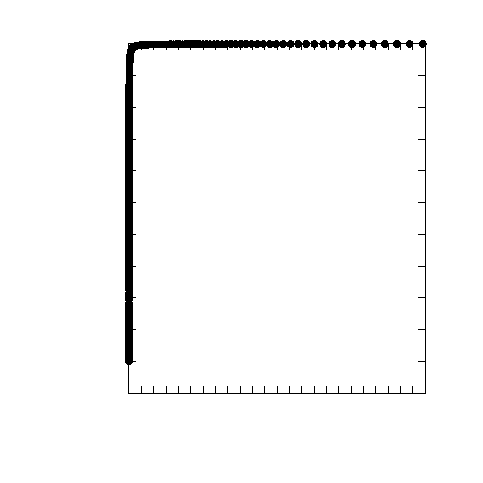
\includegraphics{akzeptanzrategrob}}%
    \gplfronttext
  \end{picture}%
\endgroup

		\end{minipage}
		\begin{minipage}{0.48\textwidth}
			% GNUPLOT: LaTeX picture with Postscript
\begingroup
  \makeatletter
  \providecommand\color[2][]{%
    \GenericError{(gnuplot) \space\space\space\@spaces}{%
      Package color not loaded in conjunction with
      terminal option `colourtext'%
    }{See the gnuplot documentation for explanation.%
    }{Either use 'blacktext' in gnuplot or load the package
      color.sty in LaTeX.}%
    \renewcommand\color[2][]{}%
  }%
  \providecommand\includegraphics[2][]{%
    \GenericError{(gnuplot) \space\space\space\@spaces}{%
      Package graphicx or graphics not loaded%
    }{See the gnuplot documentation for explanation.%
    }{The gnuplot epslatex terminal needs graphicx.sty or graphics.sty.}%
    \renewcommand\includegraphics[2][]{}%
  }%
  \providecommand\rotatebox[2]{#2}%
  \@ifundefined{ifGPcolor}{%
    \newif\ifGPcolor
    \GPcolortrue
  }{}%
  \@ifundefined{ifGPblacktext}{%
    \newif\ifGPblacktext
    \GPblacktextfalse
  }{}%
  % define a \g@addto@macro without @ in the name:
  \let\gplgaddtomacro\g@addto@macro
  % define empty templates for all commands taking text:
  \gdef\gplbacktext{}%
  \gdef\gplfronttext{}%
  \makeatother
  \ifGPblacktext
    % no textcolor at all
    \def\colorrgb#1{}%
    \def\colorgray#1{}%
  \else
    % gray or color?
    \ifGPcolor
      \def\colorrgb#1{\color[rgb]{#1}}%
      \def\colorgray#1{\color[gray]{#1}}%
      \expandafter\def\csname LTw\endcsname{\color{white}}%
      \expandafter\def\csname LTb\endcsname{\color{black}}%
      \expandafter\def\csname LTa\endcsname{\color{black}}%
      \expandafter\def\csname LT0\endcsname{\color[rgb]{1,0,0}}%
      \expandafter\def\csname LT1\endcsname{\color[rgb]{0,1,0}}%
      \expandafter\def\csname LT2\endcsname{\color[rgb]{0,0,1}}%
      \expandafter\def\csname LT3\endcsname{\color[rgb]{1,0,1}}%
      \expandafter\def\csname LT4\endcsname{\color[rgb]{0,1,1}}%
      \expandafter\def\csname LT5\endcsname{\color[rgb]{1,1,0}}%
      \expandafter\def\csname LT6\endcsname{\color[rgb]{0,0,0}}%
      \expandafter\def\csname LT7\endcsname{\color[rgb]{1,0.3,0}}%
      \expandafter\def\csname LT8\endcsname{\color[rgb]{0.5,0.5,0.5}}%
    \else
      % gray
      \def\colorrgb#1{\color{black}}%
      \def\colorgray#1{\color[gray]{#1}}%
      \expandafter\def\csname LTw\endcsname{\color{white}}%
      \expandafter\def\csname LTb\endcsname{\color{black}}%
      \expandafter\def\csname LTa\endcsname{\color{black}}%
      \expandafter\def\csname LT0\endcsname{\color{black}}%
      \expandafter\def\csname LT1\endcsname{\color{black}}%
      \expandafter\def\csname LT2\endcsname{\color{black}}%
      \expandafter\def\csname LT3\endcsname{\color{black}}%
      \expandafter\def\csname LT4\endcsname{\color{black}}%
      \expandafter\def\csname LT5\endcsname{\color{black}}%
      \expandafter\def\csname LT6\endcsname{\color{black}}%
      \expandafter\def\csname LT7\endcsname{\color{black}}%
      \expandafter\def\csname LT8\endcsname{\color{black}}%
    \fi
  \fi
    \setlength{\unitlength}{0.0500bp}%
    \ifx\gptboxheight\undefined%
      \newlength{\gptboxheight}%
      \newlength{\gptboxwidth}%
      \newsavebox{\gptboxtext}%
    \fi%
    \setlength{\fboxrule}{0.5pt}%
    \setlength{\fboxsep}{1pt}%
\begin{picture}(4320.00,4320.00)%
    \gplgaddtomacro\gplbacktext{%
      \csname LTb\endcsname%
      \put(946,704){\makebox(0,0)[r]{\strut{}$-0.1$}}%
      \put(946,1123){\makebox(0,0)[r]{\strut{}$0$}}%
      \put(946,1542){\makebox(0,0)[r]{\strut{}$0.1$}}%
      \put(946,1961){\makebox(0,0)[r]{\strut{}$0.2$}}%
      \put(946,2380){\makebox(0,0)[r]{\strut{}$0.3$}}%
      \put(946,2798){\makebox(0,0)[r]{\strut{}$0.4$}}%
      \put(946,3217){\makebox(0,0)[r]{\strut{}$0.5$}}%
      \put(946,3636){\makebox(0,0)[r]{\strut{}$0.6$}}%
      \put(946,4055){\makebox(0,0)[r]{\strut{}$0.7$}}%
      \put(1078,484){\makebox(0,0){\strut{}$0$}}%
      \put(1647,484){\makebox(0,0){\strut{}$1$}}%
      \put(2216,484){\makebox(0,0){\strut{}$2$}}%
      \put(2785,484){\makebox(0,0){\strut{}$3$}}%
      \put(3354,484){\makebox(0,0){\strut{}$4$}}%
      \put(3923,484){\makebox(0,0){\strut{}$5$}}%
    }%
    \gplgaddtomacro\gplfronttext{%
      \csname LTb\endcsname%
      \put(176,2379){\rotatebox{-270}{\makebox(0,0){\strut{}Akzeptanzrate}}}%
      \put(2500,154){\makebox(0,0){\strut{}Temperatur}}%
    }%
    \gplbacktext
    \put(0,0){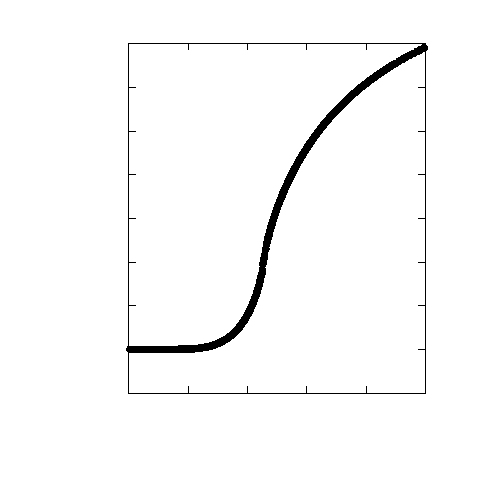
\includegraphics{akzeptanzratefein}}%
    \gplfronttext
  \end{picture}%
\endgroup

		\end{minipage}
		\caption[Akzeptanzrate in Abhängigkeit von der Temperatur]{Akzeptanzrate in Abhängigkeit von der Temperatur, gemessen bei Gitterlänge 120, mit Blocklänge 128 zur Fehlerberechnung. Die Fehler sind so klein, dass sie fast nicht sichtbar sind.}
		\label{fig:ergebnisakzeptanzrate}
	\end{figure}
	
	Der Hamiltonian verhält sich qualitativ ähnlich, siehe Bild \ref{fig:ergebnishamiltonian}. Bei geringen Temperaturen hat er den Wert $-2\cdot\text{laenge}^2$, was auf ein vollkommen homogen ausgerichtetes Gitter hinweist. Bei ca T=2,2 beträgt der Hamiltonian ca. $-1,4\cdot\text{laenge}^2$ und nähert sich dann asymptotisch null.
	
	\begin{figure}[htbp]
		\begin{minipage}{0.48\textwidth}
			% GNUPLOT: LaTeX picture with Postscript
\begingroup
  \makeatletter
  \providecommand\color[2][]{%
    \GenericError{(gnuplot) \space\space\space\@spaces}{%
      Package color not loaded in conjunction with
      terminal option `colourtext'%
    }{See the gnuplot documentation for explanation.%
    }{Either use 'blacktext' in gnuplot or load the package
      color.sty in LaTeX.}%
    \renewcommand\color[2][]{}%
  }%
  \providecommand\includegraphics[2][]{%
    \GenericError{(gnuplot) \space\space\space\@spaces}{%
      Package graphicx or graphics not loaded%
    }{See the gnuplot documentation for explanation.%
    }{The gnuplot epslatex terminal needs graphicx.sty or graphics.sty.}%
    \renewcommand\includegraphics[2][]{}%
  }%
  \providecommand\rotatebox[2]{#2}%
  \@ifundefined{ifGPcolor}{%
    \newif\ifGPcolor
    \GPcolortrue
  }{}%
  \@ifundefined{ifGPblacktext}{%
    \newif\ifGPblacktext
    \GPblacktextfalse
  }{}%
  % define a \g@addto@macro without @ in the name:
  \let\gplgaddtomacro\g@addto@macro
  % define empty templates for all commands taking text:
  \gdef\gplbacktext{}%
  \gdef\gplfronttext{}%
  \makeatother
  \ifGPblacktext
    % no textcolor at all
    \def\colorrgb#1{}%
    \def\colorgray#1{}%
  \else
    % gray or color?
    \ifGPcolor
      \def\colorrgb#1{\color[rgb]{#1}}%
      \def\colorgray#1{\color[gray]{#1}}%
      \expandafter\def\csname LTw\endcsname{\color{white}}%
      \expandafter\def\csname LTb\endcsname{\color{black}}%
      \expandafter\def\csname LTa\endcsname{\color{black}}%
      \expandafter\def\csname LT0\endcsname{\color[rgb]{1,0,0}}%
      \expandafter\def\csname LT1\endcsname{\color[rgb]{0,1,0}}%
      \expandafter\def\csname LT2\endcsname{\color[rgb]{0,0,1}}%
      \expandafter\def\csname LT3\endcsname{\color[rgb]{1,0,1}}%
      \expandafter\def\csname LT4\endcsname{\color[rgb]{0,1,1}}%
      \expandafter\def\csname LT5\endcsname{\color[rgb]{1,1,0}}%
      \expandafter\def\csname LT6\endcsname{\color[rgb]{0,0,0}}%
      \expandafter\def\csname LT7\endcsname{\color[rgb]{1,0.3,0}}%
      \expandafter\def\csname LT8\endcsname{\color[rgb]{0.5,0.5,0.5}}%
    \else
      % gray
      \def\colorrgb#1{\color{black}}%
      \def\colorgray#1{\color[gray]{#1}}%
      \expandafter\def\csname LTw\endcsname{\color{white}}%
      \expandafter\def\csname LTb\endcsname{\color{black}}%
      \expandafter\def\csname LTa\endcsname{\color{black}}%
      \expandafter\def\csname LT0\endcsname{\color{black}}%
      \expandafter\def\csname LT1\endcsname{\color{black}}%
      \expandafter\def\csname LT2\endcsname{\color{black}}%
      \expandafter\def\csname LT3\endcsname{\color{black}}%
      \expandafter\def\csname LT4\endcsname{\color{black}}%
      \expandafter\def\csname LT5\endcsname{\color{black}}%
      \expandafter\def\csname LT6\endcsname{\color{black}}%
      \expandafter\def\csname LT7\endcsname{\color{black}}%
      \expandafter\def\csname LT8\endcsname{\color{black}}%
    \fi
  \fi
    \setlength{\unitlength}{0.0500bp}%
    \ifx\gptboxheight\undefined%
      \newlength{\gptboxheight}%
      \newlength{\gptboxwidth}%
      \newsavebox{\gptboxtext}%
    \fi%
    \setlength{\fboxrule}{0.5pt}%
    \setlength{\fboxsep}{1pt}%
\begin{picture}(4320.00,4320.00)%
    \gplgaddtomacro\gplbacktext{%
      \csname LTb\endcsname%
      \put(946,704){\makebox(0,0)[r]{\strut{}$-2.5$}}%
      \put(946,1263){\makebox(0,0)[r]{\strut{}$-2$}}%
      \put(946,1821){\makebox(0,0)[r]{\strut{}$-1.5$}}%
      \put(946,2380){\makebox(0,0)[r]{\strut{}$-1$}}%
      \put(946,2938){\makebox(0,0)[r]{\strut{}$-0.5$}}%
      \put(946,3497){\makebox(0,0)[r]{\strut{}$0$}}%
      \put(946,4055){\makebox(0,0)[r]{\strut{}$0.5$}}%
      \put(1078,484){\makebox(0,0){\strut{}$0$}}%
      \put(1197,484){\makebox(0,0){\strut{}$400$}}%
      \put(1315,484){\makebox(0,0){\strut{}$800$}}%
      \put(1434,484){\makebox(0,0){\strut{}$1200$}}%
      \put(1552,484){\makebox(0,0){\strut{}$1600$}}%
      \put(1671,484){\makebox(0,0){\strut{}$2000$}}%
      \put(1789,484){\makebox(0,0){\strut{}$2400$}}%
      \put(1908,484){\makebox(0,0){\strut{}$2800$}}%
      \put(2026,484){\makebox(0,0){\strut{}$3200$}}%
      \put(2145,484){\makebox(0,0){\strut{}$3600$}}%
      \put(2263,484){\makebox(0,0){\strut{}$4000$}}%
      \put(2382,484){\makebox(0,0){\strut{}$4400$}}%
      \put(2501,484){\makebox(0,0){\strut{}$4800$}}%
      \put(2619,484){\makebox(0,0){\strut{}$5200$}}%
      \put(2738,484){\makebox(0,0){\strut{}$5600$}}%
      \put(2856,484){\makebox(0,0){\strut{}$6000$}}%
      \put(2975,484){\makebox(0,0){\strut{}$6400$}}%
      \put(3093,484){\makebox(0,0){\strut{}$6800$}}%
      \put(3212,484){\makebox(0,0){\strut{}$7200$}}%
      \put(3330,484){\makebox(0,0){\strut{}$7600$}}%
      \put(3449,484){\makebox(0,0){\strut{}$8000$}}%
      \put(3567,484){\makebox(0,0){\strut{}$8400$}}%
      \put(3686,484){\makebox(0,0){\strut{}$8800$}}%
      \put(3804,484){\makebox(0,0){\strut{}$9200$}}%
      \put(3923,484){\makebox(0,0){\strut{}$9600$}}%
    }%
    \gplgaddtomacro\gplfronttext{%
      \csname LTb\endcsname%
      \put(176,2379){\rotatebox{-270}{\makebox(0,0){\strut{}$H/\text{laenge}^2$}}}%
      \put(2500,154){\makebox(0,0){\strut{}Temperatur}}%
    }%
    \gplbacktext
    \put(0,0){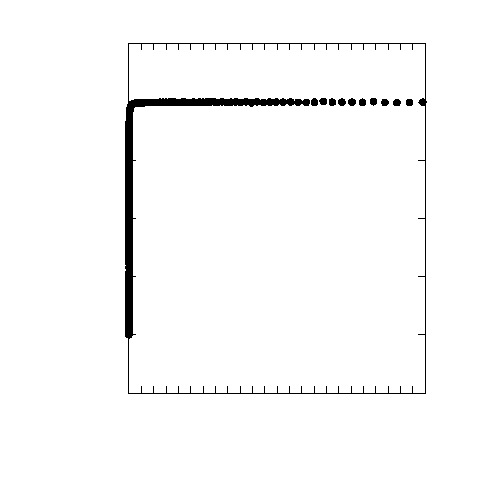
\includegraphics{hamiltoniangrob}}%
    \gplfronttext
  \end{picture}%
\endgroup

		\end{minipage}
		\begin{minipage}{0.48\textwidth}
			% GNUPLOT: LaTeX picture with Postscript
\begingroup
  \makeatletter
  \providecommand\color[2][]{%
    \GenericError{(gnuplot) \space\space\space\@spaces}{%
      Package color not loaded in conjunction with
      terminal option `colourtext'%
    }{See the gnuplot documentation for explanation.%
    }{Either use 'blacktext' in gnuplot or load the package
      color.sty in LaTeX.}%
    \renewcommand\color[2][]{}%
  }%
  \providecommand\includegraphics[2][]{%
    \GenericError{(gnuplot) \space\space\space\@spaces}{%
      Package graphicx or graphics not loaded%
    }{See the gnuplot documentation for explanation.%
    }{The gnuplot epslatex terminal needs graphicx.sty or graphics.sty.}%
    \renewcommand\includegraphics[2][]{}%
  }%
  \providecommand\rotatebox[2]{#2}%
  \@ifundefined{ifGPcolor}{%
    \newif\ifGPcolor
    \GPcolortrue
  }{}%
  \@ifundefined{ifGPblacktext}{%
    \newif\ifGPblacktext
    \GPblacktextfalse
  }{}%
  % define a \g@addto@macro without @ in the name:
  \let\gplgaddtomacro\g@addto@macro
  % define empty templates for all commands taking text:
  \gdef\gplbacktext{}%
  \gdef\gplfronttext{}%
  \makeatother
  \ifGPblacktext
    % no textcolor at all
    \def\colorrgb#1{}%
    \def\colorgray#1{}%
  \else
    % gray or color?
    \ifGPcolor
      \def\colorrgb#1{\color[rgb]{#1}}%
      \def\colorgray#1{\color[gray]{#1}}%
      \expandafter\def\csname LTw\endcsname{\color{white}}%
      \expandafter\def\csname LTb\endcsname{\color{black}}%
      \expandafter\def\csname LTa\endcsname{\color{black}}%
      \expandafter\def\csname LT0\endcsname{\color[rgb]{1,0,0}}%
      \expandafter\def\csname LT1\endcsname{\color[rgb]{0,1,0}}%
      \expandafter\def\csname LT2\endcsname{\color[rgb]{0,0,1}}%
      \expandafter\def\csname LT3\endcsname{\color[rgb]{1,0,1}}%
      \expandafter\def\csname LT4\endcsname{\color[rgb]{0,1,1}}%
      \expandafter\def\csname LT5\endcsname{\color[rgb]{1,1,0}}%
      \expandafter\def\csname LT6\endcsname{\color[rgb]{0,0,0}}%
      \expandafter\def\csname LT7\endcsname{\color[rgb]{1,0.3,0}}%
      \expandafter\def\csname LT8\endcsname{\color[rgb]{0.5,0.5,0.5}}%
    \else
      % gray
      \def\colorrgb#1{\color{black}}%
      \def\colorgray#1{\color[gray]{#1}}%
      \expandafter\def\csname LTw\endcsname{\color{white}}%
      \expandafter\def\csname LTb\endcsname{\color{black}}%
      \expandafter\def\csname LTa\endcsname{\color{black}}%
      \expandafter\def\csname LT0\endcsname{\color{black}}%
      \expandafter\def\csname LT1\endcsname{\color{black}}%
      \expandafter\def\csname LT2\endcsname{\color{black}}%
      \expandafter\def\csname LT3\endcsname{\color{black}}%
      \expandafter\def\csname LT4\endcsname{\color{black}}%
      \expandafter\def\csname LT5\endcsname{\color{black}}%
      \expandafter\def\csname LT6\endcsname{\color{black}}%
      \expandafter\def\csname LT7\endcsname{\color{black}}%
      \expandafter\def\csname LT8\endcsname{\color{black}}%
    \fi
  \fi
    \setlength{\unitlength}{0.0500bp}%
    \ifx\gptboxheight\undefined%
      \newlength{\gptboxheight}%
      \newlength{\gptboxwidth}%
      \newsavebox{\gptboxtext}%
    \fi%
    \setlength{\fboxrule}{0.5pt}%
    \setlength{\fboxsep}{1pt}%
\begin{picture}(4320.00,4320.00)%
    \gplgaddtomacro\gplbacktext{%
      \csname LTb\endcsname%
      \put(946,704){\makebox(0,0)[r]{\strut{}$-2.2$}}%
      \put(946,1076){\makebox(0,0)[r]{\strut{}$-2$}}%
      \put(946,1449){\makebox(0,0)[r]{\strut{}$-1.8$}}%
      \put(946,1821){\makebox(0,0)[r]{\strut{}$-1.6$}}%
      \put(946,2193){\makebox(0,0)[r]{\strut{}$-1.4$}}%
      \put(946,2566){\makebox(0,0)[r]{\strut{}$-1.2$}}%
      \put(946,2938){\makebox(0,0)[r]{\strut{}$-1$}}%
      \put(946,3310){\makebox(0,0)[r]{\strut{}$-0.8$}}%
      \put(946,3683){\makebox(0,0)[r]{\strut{}$-0.6$}}%
      \put(946,4055){\makebox(0,0)[r]{\strut{}$-0.4$}}%
      \put(1078,484){\makebox(0,0){\strut{}$0$}}%
      \put(1647,484){\makebox(0,0){\strut{}$1$}}%
      \put(2216,484){\makebox(0,0){\strut{}$2$}}%
      \put(2785,484){\makebox(0,0){\strut{}$3$}}%
      \put(3354,484){\makebox(0,0){\strut{}$4$}}%
      \put(3923,484){\makebox(0,0){\strut{}$5$}}%
    }%
    \gplgaddtomacro\gplfronttext{%
      \csname LTb\endcsname%
      \put(176,2379){\rotatebox{-270}{\makebox(0,0){\strut{}$H/\text{laenge}^2$}}}%
      \put(2500,154){\makebox(0,0){\strut{}Temperatur}}%
    }%
    \gplbacktext
    \put(0,0){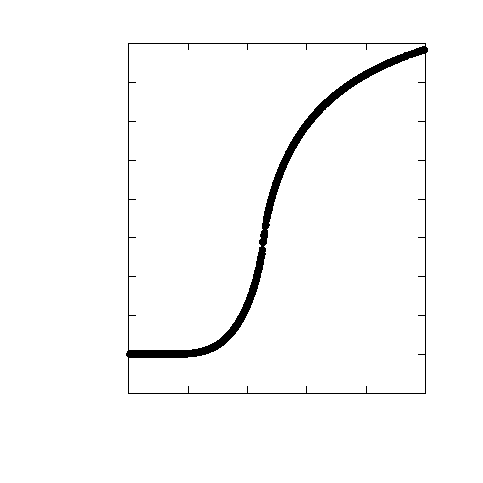
\includegraphics{hamiltonianfein}}%
    \gplfronttext
  \end{picture}%
\endgroup

		\end{minipage}
		\caption[Hamiltonian in Abhängigkeit von der Temperatur]{Hamiltonian in Abhängigkeit von der Temperatur, gemessen bei Gitterlänge 120, mit Blocklänge 128 zur Fehlerberechnung. Die Fehler sind so klein, dass sie fast nicht sichtbar sind.}
		\label{fig:ergebnishamiltonian}
	\end{figure}
	
%	Dann Akzeptanzrate von wo bis wo, mit gebootstraptem Fehler? Geht auf 1 hoch?
%	\begin{verbatim}
%	test
%	\end{verbatim}

	Die Magnetisierung verhält sich wie nach Gl. \ref{eq:magnetisierungsgleichungliteratur} erwartet: Bei geringen Temperaturen ist sie eins, danach wird sich kleiner. Bei ca. 2,2 hat sie einen starken Abfall, und nähert sich danach einem konstanten Wert größer als null an. Nach Gl. \ref{eq:magnetisierungsgleichungliteratur} wäre zu erwarten, dass der Abfall eine scharfe Kante bildet und danach die Magnetisierung null ist, dies ist allerdings aufgrund der endlichen Gittergöße nicht der Fall, wie in \cite[Abschnitt 2.3.3]{binderheermann} erläutert wird.

	
	\begin{figure}[htbp]
		\begin{minipage}{0.48\textwidth}
			% GNUPLOT: LaTeX picture with Postscript
\begingroup
  \makeatletter
  \providecommand\color[2][]{%
    \GenericError{(gnuplot) \space\space\space\@spaces}{%
      Package color not loaded in conjunction with
      terminal option `colourtext'%
    }{See the gnuplot documentation for explanation.%
    }{Either use 'blacktext' in gnuplot or load the package
      color.sty in LaTeX.}%
    \renewcommand\color[2][]{}%
  }%
  \providecommand\includegraphics[2][]{%
    \GenericError{(gnuplot) \space\space\space\@spaces}{%
      Package graphicx or graphics not loaded%
    }{See the gnuplot documentation for explanation.%
    }{The gnuplot epslatex terminal needs graphicx.sty or graphics.sty.}%
    \renewcommand\includegraphics[2][]{}%
  }%
  \providecommand\rotatebox[2]{#2}%
  \@ifundefined{ifGPcolor}{%
    \newif\ifGPcolor
    \GPcolortrue
  }{}%
  \@ifundefined{ifGPblacktext}{%
    \newif\ifGPblacktext
    \GPblacktextfalse
  }{}%
  % define a \g@addto@macro without @ in the name:
  \let\gplgaddtomacro\g@addto@macro
  % define empty templates for all commands taking text:
  \gdef\gplbacktext{}%
  \gdef\gplfronttext{}%
  \makeatother
  \ifGPblacktext
    % no textcolor at all
    \def\colorrgb#1{}%
    \def\colorgray#1{}%
  \else
    % gray or color?
    \ifGPcolor
      \def\colorrgb#1{\color[rgb]{#1}}%
      \def\colorgray#1{\color[gray]{#1}}%
      \expandafter\def\csname LTw\endcsname{\color{white}}%
      \expandafter\def\csname LTb\endcsname{\color{black}}%
      \expandafter\def\csname LTa\endcsname{\color{black}}%
      \expandafter\def\csname LT0\endcsname{\color[rgb]{1,0,0}}%
      \expandafter\def\csname LT1\endcsname{\color[rgb]{0,1,0}}%
      \expandafter\def\csname LT2\endcsname{\color[rgb]{0,0,1}}%
      \expandafter\def\csname LT3\endcsname{\color[rgb]{1,0,1}}%
      \expandafter\def\csname LT4\endcsname{\color[rgb]{0,1,1}}%
      \expandafter\def\csname LT5\endcsname{\color[rgb]{1,1,0}}%
      \expandafter\def\csname LT6\endcsname{\color[rgb]{0,0,0}}%
      \expandafter\def\csname LT7\endcsname{\color[rgb]{1,0.3,0}}%
      \expandafter\def\csname LT8\endcsname{\color[rgb]{0.5,0.5,0.5}}%
    \else
      % gray
      \def\colorrgb#1{\color{black}}%
      \def\colorgray#1{\color[gray]{#1}}%
      \expandafter\def\csname LTw\endcsname{\color{white}}%
      \expandafter\def\csname LTb\endcsname{\color{black}}%
      \expandafter\def\csname LTa\endcsname{\color{black}}%
      \expandafter\def\csname LT0\endcsname{\color{black}}%
      \expandafter\def\csname LT1\endcsname{\color{black}}%
      \expandafter\def\csname LT2\endcsname{\color{black}}%
      \expandafter\def\csname LT3\endcsname{\color{black}}%
      \expandafter\def\csname LT4\endcsname{\color{black}}%
      \expandafter\def\csname LT5\endcsname{\color{black}}%
      \expandafter\def\csname LT6\endcsname{\color{black}}%
      \expandafter\def\csname LT7\endcsname{\color{black}}%
      \expandafter\def\csname LT8\endcsname{\color{black}}%
    \fi
  \fi
    \setlength{\unitlength}{0.0500bp}%
    \ifx\gptboxheight\undefined%
      \newlength{\gptboxheight}%
      \newlength{\gptboxwidth}%
      \newsavebox{\gptboxtext}%
    \fi%
    \setlength{\fboxrule}{0.5pt}%
    \setlength{\fboxsep}{1pt}%
\begin{picture}(4320.00,4320.00)%
    \gplgaddtomacro\gplbacktext{%
      \csname LTb\endcsname%
      \put(814,704){\makebox(0,0)[r]{\strut{}$0$}}%
      \put(814,1009){\makebox(0,0)[r]{\strut{}$0.1$}}%
      \put(814,1313){\makebox(0,0)[r]{\strut{}$0.2$}}%
      \put(814,1618){\makebox(0,0)[r]{\strut{}$0.3$}}%
      \put(814,1923){\makebox(0,0)[r]{\strut{}$0.4$}}%
      \put(814,2227){\makebox(0,0)[r]{\strut{}$0.5$}}%
      \put(814,2532){\makebox(0,0)[r]{\strut{}$0.6$}}%
      \put(814,2836){\makebox(0,0)[r]{\strut{}$0.7$}}%
      \put(814,3141){\makebox(0,0)[r]{\strut{}$0.8$}}%
      \put(814,3446){\makebox(0,0)[r]{\strut{}$0.9$}}%
      \put(814,3750){\makebox(0,0)[r]{\strut{}$1$}}%
      \put(814,4055){\makebox(0,0)[r]{\strut{}$1.1$}}%
      \put(946,484){\makebox(0,0){\strut{}$0$}}%
      \put(1070,484){\makebox(0,0){\strut{}$400$}}%
      \put(1194,484){\makebox(0,0){\strut{}$800$}}%
      \put(1318,484){\makebox(0,0){\strut{}$1200$}}%
      \put(1442,484){\makebox(0,0){\strut{}$1600$}}%
      \put(1566,484){\makebox(0,0){\strut{}$2000$}}%
      \put(1690,484){\makebox(0,0){\strut{}$2400$}}%
      \put(1814,484){\makebox(0,0){\strut{}$2800$}}%
      \put(1938,484){\makebox(0,0){\strut{}$3200$}}%
      \put(2062,484){\makebox(0,0){\strut{}$3600$}}%
      \put(2186,484){\makebox(0,0){\strut{}$4000$}}%
      \put(2310,484){\makebox(0,0){\strut{}$4400$}}%
      \put(2435,484){\makebox(0,0){\strut{}$4800$}}%
      \put(2559,484){\makebox(0,0){\strut{}$5200$}}%
      \put(2683,484){\makebox(0,0){\strut{}$5600$}}%
      \put(2807,484){\makebox(0,0){\strut{}$6000$}}%
      \put(2931,484){\makebox(0,0){\strut{}$6400$}}%
      \put(3055,484){\makebox(0,0){\strut{}$6800$}}%
      \put(3179,484){\makebox(0,0){\strut{}$7200$}}%
      \put(3303,484){\makebox(0,0){\strut{}$7600$}}%
      \put(3427,484){\makebox(0,0){\strut{}$8000$}}%
      \put(3551,484){\makebox(0,0){\strut{}$8400$}}%
      \put(3675,484){\makebox(0,0){\strut{}$8800$}}%
      \put(3799,484){\makebox(0,0){\strut{}$9200$}}%
      \put(3923,484){\makebox(0,0){\strut{}$9600$}}%
    }%
    \gplgaddtomacro\gplfronttext{%
      \csname LTb\endcsname%
      \put(176,2379){\rotatebox{-270}{\makebox(0,0){\strut{}$M$}}}%
      \put(2434,154){\makebox(0,0){\strut{}Temperatur}}%
    }%
    \gplbacktext
    \put(0,0){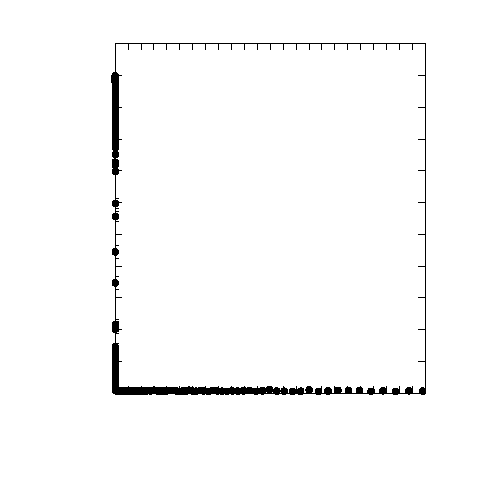
\includegraphics{magnetisierunggrob}}%
    \gplfronttext
  \end{picture}%
\endgroup

		\end{minipage}
		\begin{minipage}{0.48\textwidth}
			% GNUPLOT: LaTeX picture with Postscript
\begingroup
  \makeatletter
  \providecommand\color[2][]{%
    \GenericError{(gnuplot) \space\space\space\@spaces}{%
      Package color not loaded in conjunction with
      terminal option `colourtext'%
    }{See the gnuplot documentation for explanation.%
    }{Either use 'blacktext' in gnuplot or load the package
      color.sty in LaTeX.}%
    \renewcommand\color[2][]{}%
  }%
  \providecommand\includegraphics[2][]{%
    \GenericError{(gnuplot) \space\space\space\@spaces}{%
      Package graphicx or graphics not loaded%
    }{See the gnuplot documentation for explanation.%
    }{The gnuplot epslatex terminal needs graphicx.sty or graphics.sty.}%
    \renewcommand\includegraphics[2][]{}%
  }%
  \providecommand\rotatebox[2]{#2}%
  \@ifundefined{ifGPcolor}{%
    \newif\ifGPcolor
    \GPcolortrue
  }{}%
  \@ifundefined{ifGPblacktext}{%
    \newif\ifGPblacktext
    \GPblacktextfalse
  }{}%
  % define a \g@addto@macro without @ in the name:
  \let\gplgaddtomacro\g@addto@macro
  % define empty templates for all commands taking text:
  \gdef\gplbacktext{}%
  \gdef\gplfronttext{}%
  \makeatother
  \ifGPblacktext
    % no textcolor at all
    \def\colorrgb#1{}%
    \def\colorgray#1{}%
  \else
    % gray or color?
    \ifGPcolor
      \def\colorrgb#1{\color[rgb]{#1}}%
      \def\colorgray#1{\color[gray]{#1}}%
      \expandafter\def\csname LTw\endcsname{\color{white}}%
      \expandafter\def\csname LTb\endcsname{\color{black}}%
      \expandafter\def\csname LTa\endcsname{\color{black}}%
      \expandafter\def\csname LT0\endcsname{\color[rgb]{1,0,0}}%
      \expandafter\def\csname LT1\endcsname{\color[rgb]{0,1,0}}%
      \expandafter\def\csname LT2\endcsname{\color[rgb]{0,0,1}}%
      \expandafter\def\csname LT3\endcsname{\color[rgb]{1,0,1}}%
      \expandafter\def\csname LT4\endcsname{\color[rgb]{0,1,1}}%
      \expandafter\def\csname LT5\endcsname{\color[rgb]{1,1,0}}%
      \expandafter\def\csname LT6\endcsname{\color[rgb]{0,0,0}}%
      \expandafter\def\csname LT7\endcsname{\color[rgb]{1,0.3,0}}%
      \expandafter\def\csname LT8\endcsname{\color[rgb]{0.5,0.5,0.5}}%
    \else
      % gray
      \def\colorrgb#1{\color{black}}%
      \def\colorgray#1{\color[gray]{#1}}%
      \expandafter\def\csname LTw\endcsname{\color{white}}%
      \expandafter\def\csname LTb\endcsname{\color{black}}%
      \expandafter\def\csname LTa\endcsname{\color{black}}%
      \expandafter\def\csname LT0\endcsname{\color{black}}%
      \expandafter\def\csname LT1\endcsname{\color{black}}%
      \expandafter\def\csname LT2\endcsname{\color{black}}%
      \expandafter\def\csname LT3\endcsname{\color{black}}%
      \expandafter\def\csname LT4\endcsname{\color{black}}%
      \expandafter\def\csname LT5\endcsname{\color{black}}%
      \expandafter\def\csname LT6\endcsname{\color{black}}%
      \expandafter\def\csname LT7\endcsname{\color{black}}%
      \expandafter\def\csname LT8\endcsname{\color{black}}%
    \fi
  \fi
    \setlength{\unitlength}{0.0500bp}%
    \ifx\gptboxheight\undefined%
      \newlength{\gptboxheight}%
      \newlength{\gptboxwidth}%
      \newsavebox{\gptboxtext}%
    \fi%
    \setlength{\fboxrule}{0.5pt}%
    \setlength{\fboxsep}{1pt}%
\begin{picture}(4320.00,4320.00)%
    \gplgaddtomacro\gplbacktext{%
      \csname LTb\endcsname%
      \put(814,704){\makebox(0,0)[r]{\strut{}$0$}}%
      \put(814,1009){\makebox(0,0)[r]{\strut{}$0.1$}}%
      \put(814,1313){\makebox(0,0)[r]{\strut{}$0.2$}}%
      \put(814,1618){\makebox(0,0)[r]{\strut{}$0.3$}}%
      \put(814,1923){\makebox(0,0)[r]{\strut{}$0.4$}}%
      \put(814,2227){\makebox(0,0)[r]{\strut{}$0.5$}}%
      \put(814,2532){\makebox(0,0)[r]{\strut{}$0.6$}}%
      \put(814,2836){\makebox(0,0)[r]{\strut{}$0.7$}}%
      \put(814,3141){\makebox(0,0)[r]{\strut{}$0.8$}}%
      \put(814,3446){\makebox(0,0)[r]{\strut{}$0.9$}}%
      \put(814,3750){\makebox(0,0)[r]{\strut{}$1$}}%
      \put(814,4055){\makebox(0,0)[r]{\strut{}$1.1$}}%
      \put(946,484){\makebox(0,0){\strut{}$0$}}%
      \put(1541,484){\makebox(0,0){\strut{}$1$}}%
      \put(2137,484){\makebox(0,0){\strut{}$2$}}%
      \put(2732,484){\makebox(0,0){\strut{}$3$}}%
      \put(3328,484){\makebox(0,0){\strut{}$4$}}%
      \put(3923,484){\makebox(0,0){\strut{}$5$}}%
    }%
    \gplgaddtomacro\gplfronttext{%
      \csname LTb\endcsname%
      \put(176,2379){\rotatebox{-270}{\makebox(0,0){\strut{}$M$}}}%
      \put(2434,154){\makebox(0,0){\strut{}Temperatur}}%
    }%
    \gplbacktext
    \put(0,0){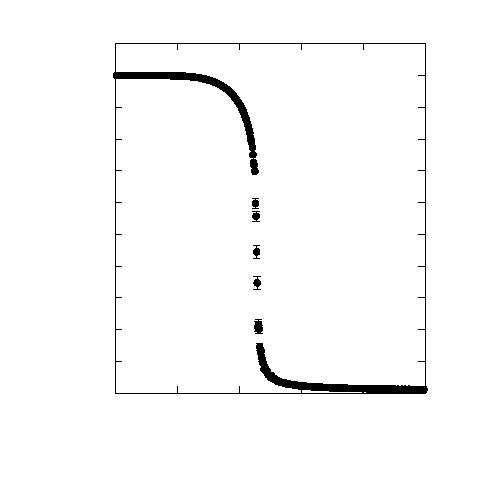
\includegraphics{magnetisierungfein}}%
    \gplfronttext
  \end{picture}%
\endgroup

		\end{minipage}
		\caption[Magnetisierung in Abhängigkeit von der Temperatur]{Magnetisierung in Abhängigkeit von der Temperatur, gemessen bei Gitterlänge 120, mit Blocklänge 128 zur Fehlerberechnung. Die Fehler sind teilweise so klein, dass sie fast nicht sichtbar sind.}
		\label{fig:ergebnismagnetisierung}
	\end{figure}	
	
	%Dann Magnetisierung: Vergleich zweier Längen, Erklärung finite size Effekts wie in Binder-Heermann erwähnt.
	In Bild \ref{fig:ergebnismagnetisierung} ist dieses Verhalten zu sehen. In Bild \ref{fig:maglaenge} ist dies noch deutlicher zu sehen, dort wird die Magnetisierung bei zwei verschiedenen Längen miteinander verglichen. Es fällt auf, dass bei kleineren Längen der Abfall der Magnetisierung weniger steil ist, sowie die Magnetisierung oberhalb des kritischen Punktes einen größeren Wert hat. Auch dies deckt sich mit den Erwartungen aus \cite[Abschnitt 2.3.3]{binderheermann}.%, ebenso wie der Vergleich zweier Längen: bei kleineren Gitterlängen ist der Abfall weniger steil und der Wert der Magnetisierung bei hohen Temperaturen größer.
	
	
	\begin{figure}[htbp]
		% GNUPLOT: LaTeX picture with Postscript
\begingroup
  \makeatletter
  \providecommand\color[2][]{%
    \GenericError{(gnuplot) \space\space\space\@spaces}{%
      Package color not loaded in conjunction with
      terminal option `colourtext'%
    }{See the gnuplot documentation for explanation.%
    }{Either use 'blacktext' in gnuplot or load the package
      color.sty in LaTeX.}%
    \renewcommand\color[2][]{}%
  }%
  \providecommand\includegraphics[2][]{%
    \GenericError{(gnuplot) \space\space\space\@spaces}{%
      Package graphicx or graphics not loaded%
    }{See the gnuplot documentation for explanation.%
    }{The gnuplot epslatex terminal needs graphicx.sty or graphics.sty.}%
    \renewcommand\includegraphics[2][]{}%
  }%
  \providecommand\rotatebox[2]{#2}%
  \@ifundefined{ifGPcolor}{%
    \newif\ifGPcolor
    \GPcolortrue
  }{}%
  \@ifundefined{ifGPblacktext}{%
    \newif\ifGPblacktext
    \GPblacktextfalse
  }{}%
  % define a \g@addto@macro without @ in the name:
  \let\gplgaddtomacro\g@addto@macro
  % define empty templates for all commands taking text:
  \gdef\gplbacktext{}%
  \gdef\gplfronttext{}%
  \makeatother
  \ifGPblacktext
    % no textcolor at all
    \def\colorrgb#1{}%
    \def\colorgray#1{}%
  \else
    % gray or color?
    \ifGPcolor
      \def\colorrgb#1{\color[rgb]{#1}}%
      \def\colorgray#1{\color[gray]{#1}}%
      \expandafter\def\csname LTw\endcsname{\color{white}}%
      \expandafter\def\csname LTb\endcsname{\color{black}}%
      \expandafter\def\csname LTa\endcsname{\color{black}}%
      \expandafter\def\csname LT0\endcsname{\color[rgb]{1,0,0}}%
      \expandafter\def\csname LT1\endcsname{\color[rgb]{0,1,0}}%
      \expandafter\def\csname LT2\endcsname{\color[rgb]{0,0,1}}%
      \expandafter\def\csname LT3\endcsname{\color[rgb]{1,0,1}}%
      \expandafter\def\csname LT4\endcsname{\color[rgb]{0,1,1}}%
      \expandafter\def\csname LT5\endcsname{\color[rgb]{1,1,0}}%
      \expandafter\def\csname LT6\endcsname{\color[rgb]{0,0,0}}%
      \expandafter\def\csname LT7\endcsname{\color[rgb]{1,0.3,0}}%
      \expandafter\def\csname LT8\endcsname{\color[rgb]{0.5,0.5,0.5}}%
    \else
      % gray
      \def\colorrgb#1{\color{black}}%
      \def\colorgray#1{\color[gray]{#1}}%
      \expandafter\def\csname LTw\endcsname{\color{white}}%
      \expandafter\def\csname LTb\endcsname{\color{black}}%
      \expandafter\def\csname LTa\endcsname{\color{black}}%
      \expandafter\def\csname LT0\endcsname{\color{black}}%
      \expandafter\def\csname LT1\endcsname{\color{black}}%
      \expandafter\def\csname LT2\endcsname{\color{black}}%
      \expandafter\def\csname LT3\endcsname{\color{black}}%
      \expandafter\def\csname LT4\endcsname{\color{black}}%
      \expandafter\def\csname LT5\endcsname{\color{black}}%
      \expandafter\def\csname LT6\endcsname{\color{black}}%
      \expandafter\def\csname LT7\endcsname{\color{black}}%
      \expandafter\def\csname LT8\endcsname{\color{black}}%
    \fi
  \fi
    \setlength{\unitlength}{0.0500bp}%
    \ifx\gptboxheight\undefined%
      \newlength{\gptboxheight}%
      \newlength{\gptboxwidth}%
      \newsavebox{\gptboxtext}%
    \fi%
    \setlength{\fboxrule}{0.5pt}%
    \setlength{\fboxsep}{1pt}%
\begin{picture}(8640.00,6480.00)%
    \gplgaddtomacro\gplbacktext{%
      \csname LTb\endcsname%
      \put(1164,1296){\makebox(0,0)[r]{\strut{}$0$}}%
      \put(1164,2268){\makebox(0,0)[r]{\strut{}$0.2$}}%
      \put(1164,3240){\makebox(0,0)[r]{\strut{}$0.4$}}%
      \put(1164,4211){\makebox(0,0)[r]{\strut{}$0.6$}}%
      \put(1164,5183){\makebox(0,0)[r]{\strut{}$0.8$}}%
      \put(1164,6155){\makebox(0,0)[r]{\strut{}$1$}}%
      \put(1296,1076){\makebox(0,0){\strut{}$1$}}%
      \put(2448,1076){\makebox(0,0){\strut{}$1.5$}}%
      \put(3600,1076){\makebox(0,0){\strut{}$2$}}%
      \put(4752,1076){\makebox(0,0){\strut{}$2.5$}}%
      \put(5903,1076){\makebox(0,0){\strut{}$3$}}%
      \put(7055,1076){\makebox(0,0){\strut{}$3.5$}}%
      \put(8207,1076){\makebox(0,0){\strut{}$4$}}%
    }%
    \gplgaddtomacro\gplfronttext{%
      \csname LTb\endcsname%
      \put(526,3725){\rotatebox{-270}{\makebox(0,0){\strut{}$M$}}}%
      \put(4751,746){\makebox(0,0){\strut{}Temperatur}}%
      \csname LTb\endcsname%
      \put(7220,5982){\makebox(0,0)[r]{\strut{}$\text{laenge}=120$}}%
      \csname LTb\endcsname%
      \put(7220,5762){\makebox(0,0)[r]{\strut{}$\text{laenge}=36$}}%
      \csname LTb\endcsname%
      \put(7220,5542){\makebox(0,0)[r]{\strut{}Theorie}}%
    }%
    \gplbacktext
    \put(0,0){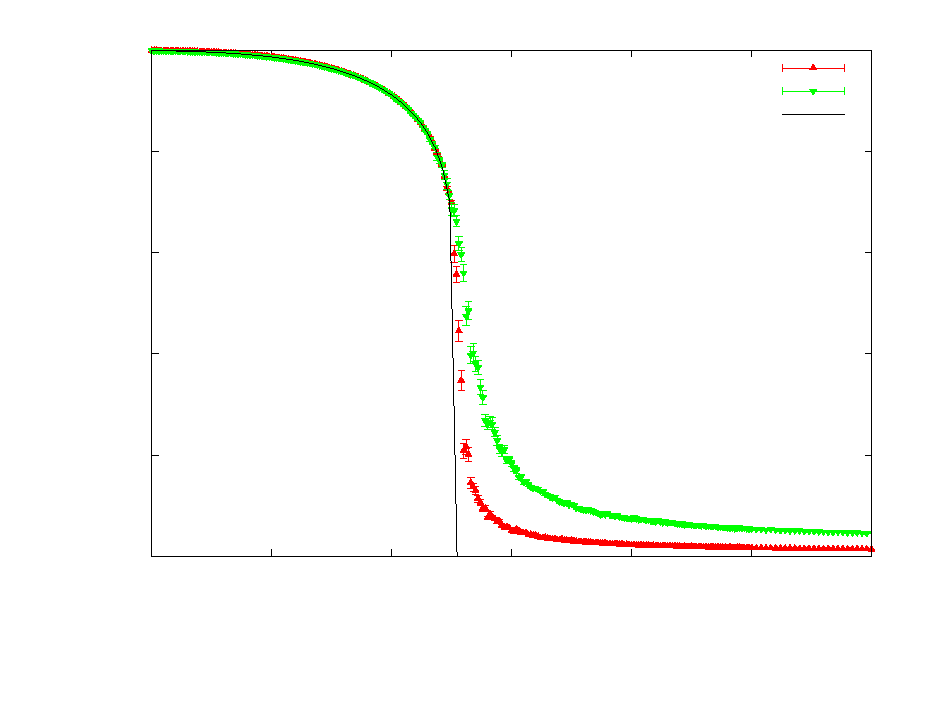
\includegraphics{magnetisierunglaenge}}%
    \gplfronttext
  \end{picture}%
\endgroup

		\label{fig:maglaenge}
		\caption[Magnetisierung bei verschiedenen Längen]{Magnetisierung bei verschiedenen Längen, Fehler gemessen mit Blocklänge 128}
	\end{figure}

	\begin{figure}[htbp]
		% GNUPLOT: LaTeX picture with Postscript
\begingroup
  \makeatletter
  \providecommand\color[2][]{%
    \GenericError{(gnuplot) \space\space\space\@spaces}{%
      Package color not loaded in conjunction with
      terminal option `colourtext'%
    }{See the gnuplot documentation for explanation.%
    }{Either use 'blacktext' in gnuplot or load the package
      color.sty in LaTeX.}%
    \renewcommand\color[2][]{}%
  }%
  \providecommand\includegraphics[2][]{%
    \GenericError{(gnuplot) \space\space\space\@spaces}{%
      Package graphicx or graphics not loaded%
    }{See the gnuplot documentation for explanation.%
    }{The gnuplot epslatex terminal needs graphicx.sty or graphics.sty.}%
    \renewcommand\includegraphics[2][]{}%
  }%
  \providecommand\rotatebox[2]{#2}%
  \@ifundefined{ifGPcolor}{%
    \newif\ifGPcolor
    \GPcolortrue
  }{}%
  \@ifundefined{ifGPblacktext}{%
    \newif\ifGPblacktext
    \GPblacktextfalse
  }{}%
  % define a \g@addto@macro without @ in the name:
  \let\gplgaddtomacro\g@addto@macro
  % define empty templates for all commands taking text:
  \gdef\gplbacktext{}%
  \gdef\gplfronttext{}%
  \makeatother
  \ifGPblacktext
    % no textcolor at all
    \def\colorrgb#1{}%
    \def\colorgray#1{}%
  \else
    % gray or color?
    \ifGPcolor
      \def\colorrgb#1{\color[rgb]{#1}}%
      \def\colorgray#1{\color[gray]{#1}}%
      \expandafter\def\csname LTw\endcsname{\color{white}}%
      \expandafter\def\csname LTb\endcsname{\color{black}}%
      \expandafter\def\csname LTa\endcsname{\color{black}}%
      \expandafter\def\csname LT0\endcsname{\color[rgb]{1,0,0}}%
      \expandafter\def\csname LT1\endcsname{\color[rgb]{0,1,0}}%
      \expandafter\def\csname LT2\endcsname{\color[rgb]{0,0,1}}%
      \expandafter\def\csname LT3\endcsname{\color[rgb]{1,0,1}}%
      \expandafter\def\csname LT4\endcsname{\color[rgb]{0,1,1}}%
      \expandafter\def\csname LT5\endcsname{\color[rgb]{1,1,0}}%
      \expandafter\def\csname LT6\endcsname{\color[rgb]{0,0,0}}%
      \expandafter\def\csname LT7\endcsname{\color[rgb]{1,0.3,0}}%
      \expandafter\def\csname LT8\endcsname{\color[rgb]{0.5,0.5,0.5}}%
    \else
      % gray
      \def\colorrgb#1{\color{black}}%
      \def\colorgray#1{\color[gray]{#1}}%
      \expandafter\def\csname LTw\endcsname{\color{white}}%
      \expandafter\def\csname LTb\endcsname{\color{black}}%
      \expandafter\def\csname LTa\endcsname{\color{black}}%
      \expandafter\def\csname LT0\endcsname{\color{black}}%
      \expandafter\def\csname LT1\endcsname{\color{black}}%
      \expandafter\def\csname LT2\endcsname{\color{black}}%
      \expandafter\def\csname LT3\endcsname{\color{black}}%
      \expandafter\def\csname LT4\endcsname{\color{black}}%
      \expandafter\def\csname LT5\endcsname{\color{black}}%
      \expandafter\def\csname LT6\endcsname{\color{black}}%
      \expandafter\def\csname LT7\endcsname{\color{black}}%
      \expandafter\def\csname LT8\endcsname{\color{black}}%
    \fi
  \fi
    \setlength{\unitlength}{0.0500bp}%
    \ifx\gptboxheight\undefined%
      \newlength{\gptboxheight}%
      \newlength{\gptboxwidth}%
      \newsavebox{\gptboxtext}%
    \fi%
    \setlength{\fboxrule}{0.5pt}%
    \setlength{\fboxsep}{1pt}%
\begin{picture}(8640.00,6480.00)%
    \gplgaddtomacro\gplbacktext{%
      \csname LTb\endcsname%
      \put(1164,1296){\makebox(0,0)[r]{\strut{}$-18$}}%
      \put(1164,1738){\makebox(0,0)[r]{\strut{}$-16$}}%
      \put(1164,2179){\makebox(0,0)[r]{\strut{}$-14$}}%
      \put(1164,2621){\makebox(0,0)[r]{\strut{}$-12$}}%
      \put(1164,3063){\makebox(0,0)[r]{\strut{}$-10$}}%
      \put(1164,3505){\makebox(0,0)[r]{\strut{}$-8$}}%
      \put(1164,3946){\makebox(0,0)[r]{\strut{}$-6$}}%
      \put(1164,4388){\makebox(0,0)[r]{\strut{}$-4$}}%
      \put(1164,4830){\makebox(0,0)[r]{\strut{}$-2$}}%
      \put(1164,5272){\makebox(0,0)[r]{\strut{}$0$}}%
      \put(1164,5713){\makebox(0,0)[r]{\strut{}$2$}}%
      \put(1164,6155){\makebox(0,0)[r]{\strut{}$4$}}%
      \put(1296,1076){\makebox(0,0){\strut{}$1$}}%
      \put(2448,1076){\makebox(0,0){\strut{}$1.5$}}%
      \put(3600,1076){\makebox(0,0){\strut{}$2$}}%
      \put(4752,1076){\makebox(0,0){\strut{}$2.5$}}%
      \put(5903,1076){\makebox(0,0){\strut{}$3$}}%
      \put(7055,1076){\makebox(0,0){\strut{}$3.5$}}%
      \put(8207,1076){\makebox(0,0){\strut{}$4$}}%
    }%
    \gplgaddtomacro\gplfronttext{%
      \csname LTb\endcsname%
      \put(526,3725){\rotatebox{-270}{\makebox(0,0){\strut{}$\dpd{M}{T}$}}}%
      \put(4751,746){\makebox(0,0){\strut{}Temperatur}}%
    }%
    \gplbacktext
    \put(0,0){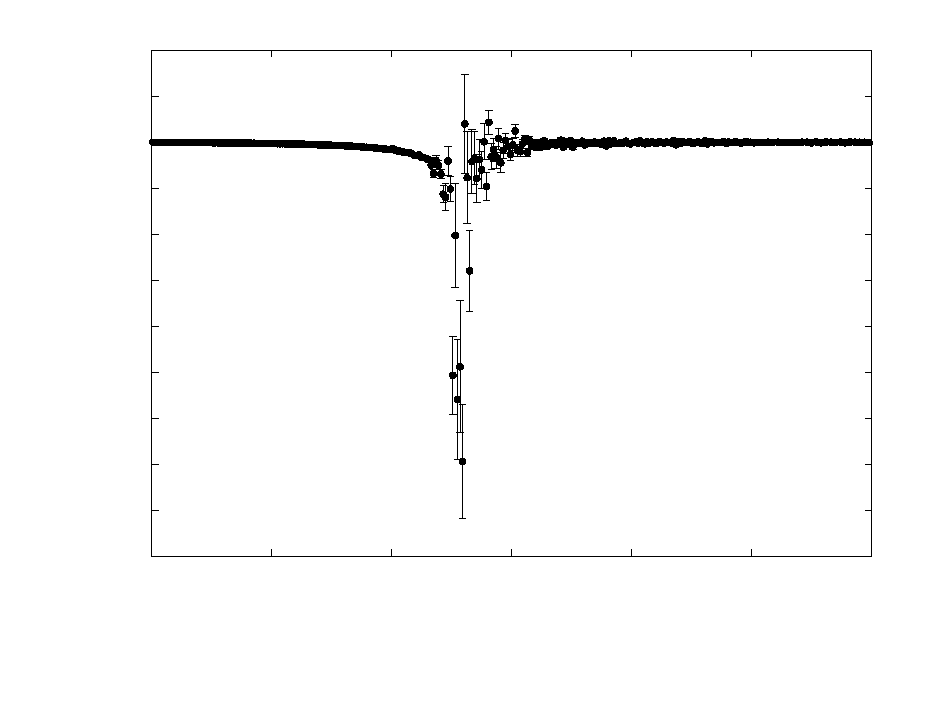
\includegraphics{ableitung120128}}%
    \gplfronttext
  \end{picture}%
\endgroup

		\label{fig:ableitung120128}
		\caption[Ableitung der Magnetisierung]{Ableitung der Magnetisierung, berechnet mit Zwei-Punkt-Formel. Fehler mit Gaußscher Fehlerfortpflanzung aus den Fehlern bei Blocklänge 128 bestimmt}
	\end{figure}
	
	In Bild \ref{fig:maglaenge} ist zusätzlich die nach Gl. \ref{eq:magnetisierungsgleichungliteratur} erwartete Magnetisierung eingezeichnet. Bis zum theoretischen kritischen Punkt, nach Gl. \ref{eq:kritischetemperatur} bei $T=2,269$, liegen alle Messdaten in ihren Fehlergrenzen auf der erwarteten Kurve, erst danach kommt es aufgrund des weniger starken Abfalls zu Abweichungen.
	
	Um den kritischen Punkt genauer zu bestimmen, wird zusätzlich mit der Zei-Punkt-Formel die Ableitung der gemessenen Magnetisierung bestimmt, siehe Bild \ref{fig:ableitung120128}. Dort wird sichtbar, dass die Änderungsrate der Magnetisierung meist sehr klein ist, nur um den kritischenb Punkt herum ist sie groß. Die größte Änderung fand im Intervall $2,285\pm0,1$ statt, dies ist minimal größer als der theoretisch erwartete kritische Punkt, die Abweichung beträgt $1,5 \sigma$. 
%	Vergleich gemessene/theoretische Magnetisierung: Nur graphisch oder auch Rechnerisch: Anpassung an Bereich mit Fehlern != 0?
	%Größte Ableitung bei 2,285 pm 0,1 bei Länge 120.
	
	%Bestimmung kritischer Punkt? Über ableitung? Oder Kumulante wie in Binder/Herrmann?
	%Theoretischer Kritischer Punkt: J*2,269
%	Messungen mit QBiG, bei denen nur die Zeit zum Durchführen von 1000 Messungen bei verschiedenen Längen und mit verschieden vielen benutzten Kernen gemessen wurde, zeigen, dass bei kleinen Längen wie 10 die benötigte Zeit mit Anzahl der Kerne sogar zunimmt. Dies ist auf den Overhead zurückzuführen.
%		
%	
%	Messungen auf Intel(R) Core(TM) i7-7500U CPU @ 2.70GHz, lcpunode01 und lcpunode02 auf QBiG.
%	
%	Parallelisierung funktioniert: Hamiltonian mit und ohne Parallelisierung gleich (Bild). siehe Bild \ref{fig:vergleichham}
%	
%	\begin{figure}[htbp]
%		% GNUPLOT: LaTeX picture with Postscript
\begingroup
  \makeatletter
  \providecommand\color[2][]{%
    \GenericError{(gnuplot) \space\space\space\@spaces}{%
      Package color not loaded in conjunction with
      terminal option `colourtext'%
    }{See the gnuplot documentation for explanation.%
    }{Either use 'blacktext' in gnuplot or load the package
      color.sty in LaTeX.}%
    \renewcommand\color[2][]{}%
  }%
  \providecommand\includegraphics[2][]{%
    \GenericError{(gnuplot) \space\space\space\@spaces}{%
      Package graphicx or graphics not loaded%
    }{See the gnuplot documentation for explanation.%
    }{The gnuplot epslatex terminal needs graphicx.sty or graphics.sty.}%
    \renewcommand\includegraphics[2][]{}%
  }%
  \providecommand\rotatebox[2]{#2}%
  \@ifundefined{ifGPcolor}{%
    \newif\ifGPcolor
    \GPcolortrue
  }{}%
  \@ifundefined{ifGPblacktext}{%
    \newif\ifGPblacktext
    \GPblacktextfalse
  }{}%
  % define a \g@addto@macro without @ in the name:
  \let\gplgaddtomacro\g@addto@macro
  % define empty templates for all commands taking text:
  \gdef\gplbacktext{}%
  \gdef\gplfronttext{}%
  \makeatother
  \ifGPblacktext
    % no textcolor at all
    \def\colorrgb#1{}%
    \def\colorgray#1{}%
  \else
    % gray or color?
    \ifGPcolor
      \def\colorrgb#1{\color[rgb]{#1}}%
      \def\colorgray#1{\color[gray]{#1}}%
      \expandafter\def\csname LTw\endcsname{\color{white}}%
      \expandafter\def\csname LTb\endcsname{\color{black}}%
      \expandafter\def\csname LTa\endcsname{\color{black}}%
      \expandafter\def\csname LT0\endcsname{\color[rgb]{1,0,0}}%
      \expandafter\def\csname LT1\endcsname{\color[rgb]{0,1,0}}%
      \expandafter\def\csname LT2\endcsname{\color[rgb]{0,0,1}}%
      \expandafter\def\csname LT3\endcsname{\color[rgb]{1,0,1}}%
      \expandafter\def\csname LT4\endcsname{\color[rgb]{0,1,1}}%
      \expandafter\def\csname LT5\endcsname{\color[rgb]{1,1,0}}%
      \expandafter\def\csname LT6\endcsname{\color[rgb]{0,0,0}}%
      \expandafter\def\csname LT7\endcsname{\color[rgb]{1,0.3,0}}%
      \expandafter\def\csname LT8\endcsname{\color[rgb]{0.5,0.5,0.5}}%
    \else
      % gray
      \def\colorrgb#1{\color{black}}%
      \def\colorgray#1{\color[gray]{#1}}%
      \expandafter\def\csname LTw\endcsname{\color{white}}%
      \expandafter\def\csname LTb\endcsname{\color{black}}%
      \expandafter\def\csname LTa\endcsname{\color{black}}%
      \expandafter\def\csname LT0\endcsname{\color{black}}%
      \expandafter\def\csname LT1\endcsname{\color{black}}%
      \expandafter\def\csname LT2\endcsname{\color{black}}%
      \expandafter\def\csname LT3\endcsname{\color{black}}%
      \expandafter\def\csname LT4\endcsname{\color{black}}%
      \expandafter\def\csname LT5\endcsname{\color{black}}%
      \expandafter\def\csname LT6\endcsname{\color{black}}%
      \expandafter\def\csname LT7\endcsname{\color{black}}%
      \expandafter\def\csname LT8\endcsname{\color{black}}%
    \fi
  \fi
    \setlength{\unitlength}{0.0500bp}%
    \ifx\gptboxheight\undefined%
      \newlength{\gptboxheight}%
      \newlength{\gptboxwidth}%
      \newsavebox{\gptboxtext}%
    \fi%
    \setlength{\fboxrule}{0.5pt}%
    \setlength{\fboxsep}{1pt}%
\begin{picture}(8640.00,6480.00)%
    \gplgaddtomacro\gplbacktext{%
      \csname LTb\endcsname%
      \put(946,704){\makebox(0,0)[r]{\strut{}$-2.2$}}%
      \put(946,1316){\makebox(0,0)[r]{\strut{}$-2$}}%
      \put(946,1929){\makebox(0,0)[r]{\strut{}$-1.8$}}%
      \put(946,2541){\makebox(0,0)[r]{\strut{}$-1.6$}}%
      \put(946,3153){\makebox(0,0)[r]{\strut{}$-1.4$}}%
      \put(946,3766){\makebox(0,0)[r]{\strut{}$-1.2$}}%
      \put(946,4378){\makebox(0,0)[r]{\strut{}$-1$}}%
      \put(946,4990){\makebox(0,0)[r]{\strut{}$-0.8$}}%
      \put(946,5603){\makebox(0,0)[r]{\strut{}$-0.6$}}%
      \put(946,6215){\makebox(0,0)[r]{\strut{}$-0.4$}}%
      \put(1078,484){\makebox(0,0){\strut{}$0$}}%
      \put(2511,484){\makebox(0,0){\strut{}$1$}}%
      \put(3944,484){\makebox(0,0){\strut{}$2$}}%
      \put(5377,484){\makebox(0,0){\strut{}$3$}}%
      \put(6810,484){\makebox(0,0){\strut{}$4$}}%
      \put(8243,484){\makebox(0,0){\strut{}$5$}}%
    }%
    \gplgaddtomacro\gplfronttext{%
      \csname LTb\endcsname%
      \put(176,3459){\rotatebox{-270}{\makebox(0,0){\strut{}$H/\text{laenge}^2$}}}%
      \put(4660,154){\makebox(0,0){\strut{}Temperatur}}%
      \csname LTb\endcsname%
      \put(4642,6042){\makebox(0,0)[r]{\strut{}zeilenweise durchgehen}}%
      \csname LTb\endcsname%
      \put(4642,5822){\makebox(0,0)[r]{\strut{}Schachbrettmuster parallel}}%
    }%
    \gplbacktext
    \put(0,0){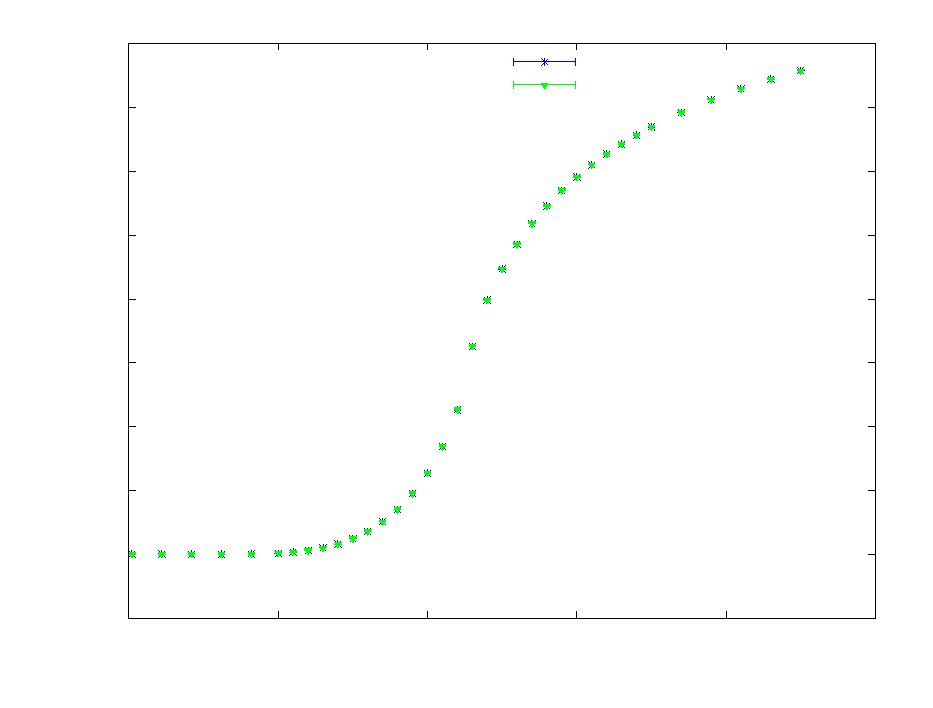
\includegraphics{vergleichham}}%
    \gplfronttext
  \end{picture}%
\endgroup

%		\label{fig:vergleichham}
%		\caption{Hamiltonian bei drei verschiedenen Methoden der Messreihenfolge bei verschiedenen Temperaturen}
%	\end{figure}
%	
%	Akzeptanzrate: für geringe Temperaturen fast null, steigt für höhere Temperaturen, bildet Plateau? siehe Bild \ref{fig:akzeptanzratenaiv}
%	
%	\begin{figure}[htbp]
%		\include{Bilder/akzeptanzratenaiv}
%		\label{fig:akzeptanzratenaiv}
%		\caption{Akzeptanzrate mit naiv berechneten Fehlern bei verschiedenen Temperaturen}
%	\end{figure}
%	
%	Magnetisierung: Für kleine Temperaturen 1 mit geringem Fehler, wird zwischen T=1,5 und T=3 kleiner, dabei größere Fehler, bei hohen Temperaturen Magnetisierung fast null mit kleinem Fehler. Vergleich mit erwartetem Wert in Bild \ref{fig:magnetisierungbootstrap-l-128}.
%	Kritischer Punkt für ${J=1:}\quad {T=2,269}$ nach Gl. \ref{eq:kritischetemperatur}, durch Ableitung (Bild) bestimmt zu $T=2,303\pm0,015$. Fehler, da kritischer Punkt in Region zwischen Wert und den nächsten Stützstellen liegen muss.
%	Unterhalb kritischer Punkt: Keinen Unterschied zu Gleichung \ref{eq:magnetisierungsgleichungliteratur}. Passt gut zu Ergebnis, Verhalten wie erwartet.
%	Oberhalb kritischer Punkt: weicht von Ergebnis aus Literatur ab, da Gitter endlich ist. Abweichung wird mit größerer Gitterlänge kleiner.
%	
%	
%	\begin{figure}[htbp]
%		\include{Bilder/magnetisierungbootstrap-l-128}
%		\label{fig:magnetisierungbootstrap-l-128}
%		\caption{Magnetisierung bei verschiedenen Temperaturen, Fehler mit Bootstrapping bei Blocklänge 128 berechnet, Vergleich mit erwarteter Magnetisierung, Gitterlänge 50}
%	\end{figure}
%		
%	Parallelisierung: Tabelle oder Bild mit Cores/Zeit.
	%Anhang
	\listoffigures
	%\listoftables
	
	
	
	\printbibliography[heading=bibintoc]
\end{document}

%\chapter{Umsetzung}
%	\section{Initialisierung und Thermalisierung}
%	Gitter, Hamiltonian, Thermalisierungsschwelle
%	
%	Gitter mit zwei for-schleifen füllen, Mersenne-Twister, der auf +-1 zugeordnet wird.
%	Hamiltonian durch Gitterdurchgang mit zwei Schleifen nach Formel \ref{eq:hamiltonianising}
%	
%	Sweep: geht gesamtes Gitter durch, führt Metropolis Update durch.
%	
%	Parallelisiert: Durchgehen in "Schachbrettmuster", erst alle schwarzen und dann alle weißen Punkte, da zum Aktualisieren der schwarzen Punkte nur alle weißen benötigt werden, somit alle Schwarzen gleichzeitig aktualisiert werden können und umgekehrt.
%	
%	Durchgang mit Schachbrettmuster dauert ca. 25 \% länger, aber beim parallelisieren geht es schon mit zwei Kernen 20 \% schneller. 
%	
%	Vergleich der Daten zeigt: Im Mittel kommt bei allen Methoden dasselbe Ergebnis heraus. \ref{fig:vergleichhamiltoniansweep}
%	
%	\begin{figure}[http]
%	\input{Bilder/Vergleichham}
%	\label{fig:vergleichhamiltoniansweep}
%		\caption{Vergleich der Mittelwerte über 10000 Messungen des Hamiltonians bei verschiedenen Methoden, das Gitter durchzugehen. Laenge=50}
%	\end{figure}
%	
%	Thermalisierung:
%	 
%	Vergleichen von Hamiltonian vor und nach sweep, solange sweeps, bis Energie sich nicht mehr verringert. Bilder?
%	Geändert, da Probleme mit Springen bei der Magnetisierung auftauchen: Anfangs Thermalisierung mit vielen sweeps (10000), danach Thermalisierung auf Basis des Gitters der vorherigen Temperatur mit (5000) Sweeps
%	
%	Ausgabe mit x, y Position, Spin in txt Datei, mit gnuplot als Heatmap plotten.
%	Verhalten: Bei niedrigen Temperaturen nur ein großer, einfarbiger Bezirk, dann bei höheren Temperaturen einige Punkte mit anderer Farbe, bei hohen Temperaturen nur Rauschen.
%	
%	\begin{figure}
%	\begin{minipage}{0.48\textwidth}
%		\input{Bilder/Gitter/gitter-laenge0050-t000.tex}
%	\end{minipage}
%	\begin{minipage}{0.48\textwidth}
%		\input{Bilder/Gitter/gitter-laenge0050-t100.tex}
%	\end{minipage}
%	\begin{minipage}{0.48\textwidth}
%		\input{Bilder/Gitter/gitter-laenge0050-t250.tex}
%	\end{minipage}
%	\caption{Gitter bei verschiedenen Temperaturen}
%	\label{fig:gitter}
%	\end{figure}
%	
%	\section{Messungen}
%	\subsection{Akzeptanzrate}
%	Beim Sweep wird jede Veränderung gezählt, am Ende wird Veränderungen/laenge/laenge in Datei geschrieben. Prozentuale Veränderung.
%	Parallelisieren: Zwischenvariable für jeden Thread. Bild, erst gering, dann steil steigend, flacht ab, bildet Plateau.
%	\begin{figure}
%		\input{Bilder/akzeptanzratenaiv.tex}
%		\label{fig:akzeptanznaiv}
%		\caption{Die Akzeptanzrate bei 10000 Messungen je Temperatur mit Laenge 50}
%	\end{figure}
%	Bei welchen Temperaturen?
%	\subsection{Magnetisierung}
%	Magnetisierung= Abs(Summe über alle Spins im Gitter)
%	
%	Bilder
%	
%	-Bei kleinen Temperaturen, unterhalb von T ungefähr 0,7, ist die
%	 Magnetisierung konstant 1, mit sehr geringen Abweichungen.
%	 
%	 -Zwischen ca. 0,7 und ca. 2,5 nimmt die Magnetisierung ab, springt jedoch
%	 immer wieder zwischen stärkeren und schwächeren Magnetisierungen hin und
%	 her. Dies wird erst ab einer gewissen Gitterlänge sichtbar, bei kleineren
%	 Gitterlängen (ausprobiert habe ich es mit 10), ist die Abnahme viel weniger
%	 sprunghaft. In diesem Bereich ist die Standardabweichung der Messungen recht
%	 groß.
%	 
%	 -Bei größeren Temperaturen, oberhalb von ca. 2,5, ist die Magnetisierung
%	 annähernd konstant und fast null. Der relative Fehler ist in diesem Bereich
%	 recht groß, jedoch ist der absolute Fehler, genau wie der Messwert, klein.
%	 
%	 Behoben durch bessere Thermalisierung: bei geringeren Temperaturen konstant 1 mit geringen Fehlern, 
%	 um T=2 herum Abfall, steiler, je länger das Gitter ist, mit recht großen Fehlern, bei hohen Temperaturen konstant niedrige Magnetisierung mit größerem Fehler als bei niedriger Temperatur. (Bild)
%	 
%	 theoretischer Kritischer Punkt für $J=1:\quad T=2,269$
%	 Bestimmung: Unstetigkeit in Magnetisierung bei kritischem Punkt erwartet, d.h. Pol in der Ableitung. 
%	 Mit 2-Punkt-Formel Ableitung bestimmen, Extremum: kritischer Punkt muss zwischen den beiden Nachbarn liegen. Ergebnis für l=128: Kritischer Punkt bei $T=2,303\pm0,015$.
%	 	\begin{figure}
%	 		\input{Bilder/ableitung.tex}
%	 		\label{fig:ableitung}
%	 		\caption{Ableitung der Daten aus l=128 mit 2-Punkt-Formel}
%	 	\end{figure}
%	 	
%	 
%	 Temperatur durch Autokorrelation, durch Bootstrapping mit blocking ausgleichen. 
%	 Zuerst Fehler, da Replika falsch verstanden, danach klare Änderung vom Fehler mit l (Bild).
%	 
%	 Magnetisierung mit Bootstrap: Bild, kleinerer Fehler, Fehler bei Phasenübergang größer als darunter/darüber.
%	\begin{figure}
%		\input{Bilder/magnetisierungbootstrap-l-128.tex}
%		\label{fig:magnetisierungbootstrap-l-128}
%		\caption{Die Magnetisierung bei 10000 Messungen je Temperatur mit Laenge 50, Bootstrapping von Daten mit Blocklänge 128}
%	\end{figure}
%		
%	Parallelisieren, indem Replica parallel gezogen werden, jedes Replica in array geschrieben, danach nur Mittelwert und Varianz über Array berechnen.
%	Vergleich: Mittelwerte gleich.
%	\begin{figure}
%		\input{Bilder/vergleichbootstrap-l-128.tex}
%		\label{fig:bootstrapparallel-l-128}
%		\caption{Die Magnetisierung bei 10000 Messungen je Temperatur mit Laenge 50, Bootstrapping von Daten mit Blocklänge 128, Vergleich von parallel und nicht paralleler Funktion}
%	\end{figure}	
